%===================================================================================
\chapter{Description of the SUNMatrix module}\label{s:sunmatrix}
%===================================================================================
\index{SUNMatrix@\texttt{SUNMatrix} module}
% This is a shared SUNDIALS TEX file with description of
% the generic sunmatrix abstraction
%
For problems that involve direct methods for solving linear systems,
the {\sundials} solvers not only operate on generic vectors, but also
on generic matrices (of type \Id{SUNMatrix}), through a set of
operations defined by the particular {\sunmatrix} implementation.
Users can provide their own specific implementation of the
{\sunmatrix} module, particularly in cases where they provide their
own {\nvector} and/or linear solver modules, and require matrices that
are compatible with those implementations.  Alternately, we provide three
{\sunmatrix} implementations: dense, banded, and sparse.  The
generic operations are described below, and descriptions of the
implementations provided with {\sundials} follow.

% ====================================================================
\section{The SUNMatrix API}
\label{s:sunmatrix_api}
% ====================================================================

The {\sunmatrix} API can be grouped into two sets of functions:
the core matrix operations, and utility functions. Section \ref{ss:sunmatrix_functions}
lists the core operations, while Section \ref{ss:sunmatrix_utilities} lists
the utility functions.

%==============================================================================
\subsection{SUNMatrix core functions}\label{ss:sunmatrix_functions}

The generic \id{SUNMatrix} object defines the following set of core operations:

\ucfunctionf{SUNMatGetID}
{
  id = SUNMatGetID(A);
}
{
  Returns the type identifier for the matrix \id{A}. It is used to determine the
  matrix implementation type (e.g.~dense, banded, sparse,\ldots) from the abstract
  \id{SUNMatrix} interface.  This is used to assess compatibility with
  {\sundials}-provided linear solver implementations.
}
{
  \begin{args}[c]
  \item[A] (\id{SUNMatrix}) a {\sunmatrix} object
  \end{args}
}
{
  A \id{SUNMATRIX\_ID}, possible values are given in the Table \ref{t:matrixIDs}.
}
{}

\ucfunctionfl{SUNMatClone}
{
  B = SUNMatClone(A);
}
{
  Creates a new \id{SUNMatrix} of the same type as an existing matrix
  \id{A} and sets the {\em ops} field. It does not copy the matrix, but
  rather allocates storage for the new matrix.
}
{
  \begin{args}[c]
  \item[A] (\id{SUNMatrix}) a {\sunmatrix} object
  \end{args}
}
{
  \id{SUNMatrix}
}
{}
{
  type(SUNMatrix), pointer :: B\\
  B => FSUNMatClone(A)
}

\ucfunctionf{SUNMatDestroy}
{
  SUNMatDestroy(A);
}
{
  Destroys \id{A} and frees memory allocated for its internal data.
}
{
  \begin{args}[c]
  \item[A] (\id{SUNMatrix}) a {\sunmatrix} object
  \end{args}
}
{}
{}

\ucfunctionfl{SUNMatSpace}
{
  ier = SUNMatSpace(A, \&lrw, \&liw);
}
{
  Returns the storage requirements for the matrix \id{A}. \id{lrw}
  is a \id{long int} containing the number of realtype words
  and \id{liw} is a \id{long int} containing the number of integer
  words.
}
{
  \begin{args}[c]
  \item[A] (\id{SUNMatrix}) a {\sunmatrix} object
  \item[lrw] (\id{sunindextype*}) the number of realtype words
  \item[liw] (\id{sunindextype*}) the number of integer words
  \end{args}
}
{}
{
  This function is advisory only, for use in determining a user's total
  space requirements; it could be a dummy function in a user-supplied
  {\sunmatrix} module if that information is not of interest.
}
{
  integer(c\_long) :: lrw(1), liw(1)\\
  ier = FSUNMatSpace(A, lrw, liw)
}

\ucfunctionf{SUNMatZero}
{
  ier = SUNMatZero(A);
}
{
  Performs the operation $A_{ij} = 0$ for all entries of the matrix $A$.
}
{
  \begin{args}[c]
  \item[A] (\id{SUNMatrix}) a {\sunmatrix} object
  \end{args}
}
{
  A {\sunmatrix} return code of type \id{int} denoting success/failure
}
{}

\ucfunctionf{SUNMatCopy}
{
  ier = SUNMatCopy(A,B);
}
{
  Performs the operation $B_{ij} = A_{i,j}$ for all entries of the matrices
  $A$ and $B$.
}
{
  \begin{args}[c]
  \item[A] (\id{SUNMatrix}) a {\sunmatrix} object
  \item[B] (\id{SUNMatrix}) a {\sunmatrix} object
  \end{args}
}
{
  A {\sunmatrix} return code of type \id{int} denoting success/failure
}
{}

\ucfunctionf{SUNMatScaleAdd}
{
  ier = SUNMatScaleAdd(c, A, B);
}
{
  Performs the operation $A = cA + B$.
}
{
  \begin{args}[c]
  \item[c] (\id{realtype}) constant that scales \id{A}
  \item[A] (\id{SUNMatrix}) a {\sunmatrix} object
  \item[B] (\id{SUNMatrix}) a {\sunmatrix} object
  \end{args}
}
{
  A {\sunmatrix} return code of type \id{int} denoting success/failure
}
{}

\ucfunctionf{SUNMatScaleAddI}
{
  ier = SUNMatScaleAddI(c, A);
}
{
  Performs the operation $A = cA + I$.
}
{
  \begin{args}[c]
  \item[c] (\id{realtype}) constant that scales \id{A}
  \item[A] (\id{SUNMatrix}) a {\sunmatrix} object
  \end{args}
}
{
  A {\sunmatrix} return code of type \id{int} denoting success/failure
}
{}

\ucfunctionf{SUNMatMatvecSetup}
{
  ier = SUNMatMatvecSetup(A);
}
{
  Performs any setup necessary to perform a matrix-vector product.
  It is useful for SUNMatrix implementations which need to prepare
  the matrix itself, or communication structures before performing
  the matrix-vector product.
}
{
  \begin{args}[A]
  \item[A] (\id{SUNMatrix}) a {\sunmatrix} object
  \end{args}
}
{
  A {\sunmatrix} return code of type \id{int} denoting success/failure
}
{}

\ucfunctionf{SUNMatMatvec}
{
  ier = SUNMatMatvec(A, x, y);
}
{
  Performs the matrix-vector product operation, $y = Ax$. It should
  only be called with vectors \id{x} and \id{y} that are compatible with
  the matrix \id{A} -- both in storage type and dimensions.
}
{
  \begin{args}[A]
  \item[A] (\id{SUNMatrix}) a {\sunmatrix} object
  \item[x] (\id{N\_Vector}) a {\nvector} object
  \item{y} (\id{N\_Vector}) an output {\nvector} object
  \end{args}
}
{
  A {\sunmatrix} return code of type \id{int} denoting success/failure
}
{}


%==============================================================================
\subsection{SUNMatrix utility functions}\label{ss:sunmatrix_utilities}

To aid in the creation of custom {\sunmatrix} modules the generic {\sunmatrix}
module provides two utility functions \id{SUNMatNewEmpty} and
\id{SUNMatVCopyOps}.

\ucfunctionf{SUNMatNewEmpty}
{
  A = SUNMatNewEmpty();
}
{
  The function \Id{SUNMatNewEmpty} allocates a new generic {\sunmatrix} object
  and initializes its content pointer and the function pointers in the
  operations structure to \id{NULL}.
}
{}
{
  This function returns a \id{SUNMatrix} object. If an error occurs when
  allocating the object, then this routine will return \id{NULL}.
}
{}

\ucfunctionf{SUNMatFreeEmpty}
{
  SUNMatFreeEmpty(A);
}
{
  This routine frees the generic \id{SUNMatrix} object, under the assumption that any
  implementation-specific data that was allocated within the underlying content structure
  has already been freed. It will additionally test whether the ops pointer is \id{NULL},
  and, if it is not, it will free it as well.
}
{
  \begin{args}[A]
  \item[A] (\id{SUNMatrix}) a \id{SUNMatrix} object
  \end{args}
}
{}
{}

\ucfunctionf{SUNMatCopyOps}
{
  retval = SUNMatCopyOps(A, B);
}
{
  The function \Id{SUNMatCopyOps} copies the function pointers in the \id{ops}
  structure of \id{A} into the \id{ops} structure of \id{B}.
}
{
  \begin{args}[A]
  \item[A] (\id{SUNMatrix}) the matrix to copy operations from
  \item[B] (\id{SUNMatrix}) the matrix to copy operations to
  \end{args}
}
{
  This returns \id{0} if successful and a non-zero value if either of the inputs
  are \id{NULL} or the \id{ops} structure of either input is \id{NULL}.
}
{}


%==============================================================================
\subsection{SUNMatrix return codes}\label{ss:sunmatrix_ReturnCodes}

The functions provided to {\sunmatrix} modules within the
{\sundials}-provided {\sunmatrix} implementations utilize a common
set of return codes, shown in Table \ref{t:sunmatrixerr}. These adhere
to a common pattern: 0 indicates success, and a negative value
indicates a failure. The actual values of each return code are
primarily to provide additional information to the user in case of
a failure.

\newlength{\AColOne}
\settowidth{\AColOne}{\id{SUNMAT\_MATVEC\_SETUP\_REQUIRED}}
\newlength{\AColTwo}
\settowidth{\AColTwo}{\id{Value}}
\newlength{\AColThree}
\setlength{\AColThree}{\textwidth}
\addtolength{\AColThree}{-0.5in}
\addtolength{\AColThree}{-\AColOne}
\addtolength{\AColThree}{-\AColTwo}

\tablecaption{Description of the \id{SUNMatrix} return codes}\label{t:sunmatrixerr}
\tablehead{\hline {\rule{0mm}{5mm}}{\bf Name} & {\bf Value} & {\bf Description} \\[3mm] \hline\hline}
\tabletail{\hline \multicolumn{3}{|r|}{\small\slshape continued on next page} \\ \hline}
\begin{xtabular}{|p{\AColOne}|p{\AColTwo}|p{\AColThree}|}
%%
\id{SUNMAT\_SUCCESS} & \id{0} & successful call or converged solve
\\[1mm]
%%
\id{SUNMAT\_ILL\_INPUT} & \id{-701} & an illegal input has been provided to the function
\\[1mm]
%%
\id{SUNMAT\_MEM\_FAIL} & \id{-702} & failed memory access or allocation
\\[1mm]
%%
\id{SUNMAT\_OPERATION\_FAIL} & \id{-703} & a SUNMatrix operation returned nonzero
\\
%%
\id{SUNMAT\_MATVEC\_SETUP\_REQUIRED} & \id{-704} & the \id{SUNMatMatvecSetup} routine
needs to be called before calling \id{SUNMatMatvec}
\\
\hline
\end{xtabular}
\bigskip


%==============================================================================
\subsection{SUNMatrix identifiers}\label{ss:sunmatrix_identifiers}

Each {\sunmatrix} implementation included in {\sundials} has a unique
identifier specified in enumeration and shown in Table \ref{t:matrixIDs}.
It is recommended that a user-supplied {\sunmatrix} implementation use the
\id{SUNMATRIX\_CUSTOM} identifier.

\begin{table}
\centering
\caption{Identifiers associated with matrix kernels supplied with {\sundials}.}
\label{t:matrixIDs}
\medskip
\begin{tabular}{|l|l|c|}
\hline
{\bf Matrix ID} & {\bf Matrix type} & {\bf ID Value} \\
\hline
SUNMATRIX\_DENSE      & Dense $\id{M} \times \id{N}$ matrix               & 0 \\
SUNMATRIX\_BAND       & Band $\id{M} \times \id{M}$ matrix                & 1 \\
SUNMATRIX\_SPARSE     & Sparse (CSR or CSC) $\id{M} \times \id{N}$ matrix & 2 \\
SUNMATRIX\_SLUNRLOC   & Adapter for the {\superludist} \id{SuperMatrix}   & 3 \\
SUNMATRIX\_CUSTOM     & User-provided custom matrix                       & 4 \\
\hline
\end{tabular}
\end{table}


%==============================================================================
\subsection{Compatibility of SUNMatrix modules}\label{ss:sunmatrix_compatibility}

We note that not all {\sunmatrix} types are compatible with all
{\nvector} types provided with {\sundials}.  This is primarily due to
the need for compatibility within the \id{SUNMatMatvec} routine;
however, compatibility between {\sunmatrix} and {\nvector}
implementations is more crucial when considering their interaction
within {\sunlinsol} objects, as will be described in more detail in
Chapter \ref{s:sunlinsol}.  More specifically, in Table
\ref{t:matrix-vector} we show the matrix interfaces available as
{\sunmatrix} modules, and the compatible vector implementations.

\tablecaption{{\sundials} matrix interfaces and vector
             implementations that can be used for each.}\label{t:matrix-vector}
\tablehead{\hline \multicolumn{1}{|p{1.5cm}|}{{Matrix Interface}} &
                  \multicolumn{1}{p{0.7cm}|}{{Serial}} &
                  \multicolumn{1}{p{1.1cm}|}{{Parallel (MPI)}} &
                  \multicolumn{1}{p{1.3cm}|}{{OpenMP}} &
                  \multicolumn{1}{p{1.3cm}|}{{pThreads}} &
                  \multicolumn{1}{p{0.9cm}|}{{{\hypre} Vec.}} &
                  \multicolumn{1}{p{0.9cm}|}{{{\petsc} Vec.}} &
                  \multicolumn{1}{p{0.8cm}|}{{{\cuda}}} &
                  \multicolumn{1}{p{0.8cm}|}{{{\raja}}} &
                  \multicolumn{1}{p{1.1cm}|}{{User Suppl.}} \\ \hline }
\tabletail{\hline \multicolumn{10}{|r|}{\small\slshape continued on next page} \\ \hline}
{\renewcommand{\arraystretch}{1.2}
\begin{xtabular}{|l|c|c|c|c|c|c|c|c|c|}
    Dense         &  \cm     &           & \cm      &  \cm       &             &          &          &          & \cm      \\
    Band          &  \cm     &           & \cm      &  \cm       &             &          &          &          & \cm      \\
    Sparse        &  \cm     &           & \cm      &  \cm       &             &          &          &          & \cm      \\
    SLUNRloc      &  \cm     & \cm       & \cm      &  \cm       & \cm         &  \cm     &          &          & \cm      \\
    User supplied &  \cm     & \cm       & \cm      &  \cm       & \cm         &  \cm     & \cm      & \cm      & \cm      \\
    \hline
\end{xtabular}
}
\bigskip


\subsection{The generic SUNMatrix module implementation}\label{ss:sunmatrix_implmentation}

The generic \ID{SUNMatrix} type has been modeled after the
object-oriented style of the generic \id{N\_Vector} type.
Specifically, a generic \ID{SUNMatrix} is a pointer to a structure
that has an implementation-dependent {\em content} field containing
the description and actual data of the matrix, and an {\em ops} field
pointing to a structure with generic matrix operations.
The type \id{SUNMatrix} is defined as
%%
%%
\begin{verbatim}
typedef struct _generic_SUNMatrix *SUNMatrix;

struct _generic_SUNMatrix {
    void *content;
    struct _generic_SUNMatrix_Ops *ops;
};
\end{verbatim}
%%
%%
The \id{\_generic\_SUNMatrix\_Ops} structure is essentially a list of pointers to
the various actual matrix operations, and is defined as
%%
\begin{verbatim}
struct _generic_SUNMatrix_Ops {
  SUNMatrix_ID (*getid)(SUNMatrix);
  SUNMatrix    (*clone)(SUNMatrix);
  void         (*destroy)(SUNMatrix);
  int          (*zero)(SUNMatrix);
  int          (*copy)(SUNMatrix, SUNMatrix);
  int          (*scaleadd)(realtype, SUNMatrix, SUNMatrix);
  int          (*scaleaddi)(realtype, SUNMatrix);
  int          (*matvecsetup)(SUNMatrix)
  int          (*matvec)(SUNMatrix, N_Vector, N_Vector);
  int          (*space)(SUNMatrix, long int*, long int*);
};
\end{verbatim}


The generic {\sunmatrix} module defines and implements the matrix operations
acting on \id{SUNMatrix} objects.
These routines are nothing but wrappers for the matrix operations defined by
a particular {\sunmatrix} implementation, which are accessed through the {\em ops}
field of the \id{SUNMatrix} structure. To illustrate this point we
show below the implementation of a typical matrix operation from the
generic {\sunmatrix} module, namely \id{SUNMatZero}, which sets all
values of a matrix \id{A} to zero, returning a flag denoting a
successful/failed operation:
%%
%%
\begin{verbatim}
int SUNMatZero(SUNMatrix A)
{
  return((int) A->ops->zero(A));
}
\end{verbatim}
%%
%%
Section \ref{ss:sunmatrix_functions} contains a complete list of all matrix operations
defined by the generic {\sunmatrix} module.

The Fortran 2003 interface provides a \id{bind(C)} derived-type for the
\id{\_generic\_SUNMatrix} and the \id{\_generic\_SUNMatrix\_Ops} structures.
Their definition is given below.
%%
%%
\begin{verbatim}
 type, bind(C), public :: SUNMatrix
  type(C_PTR), public :: content
  type(C_PTR), public :: ops
 end type SUNMatrix

 type, bind(C), public :: SUNMatrix_Ops
  type(C_FUNPTR), public :: getid
  type(C_FUNPTR), public :: clone
  type(C_FUNPTR), public :: destroy
  type(C_FUNPTR), public :: zero
  type(C_FUNPTR), public :: copy
  type(C_FUNPTR), public :: scaleadd
  type(C_FUNPTR), public :: scaleaddi
  type(C_FUNPTR), public :: matvecsetup
  type(C_FUNPTR), public :: matvec
  type(C_FUNPTR), public :: space
 end type SUNMatrix_Ops
\end{verbatim}


%==============================================================================
\subsection{Implementing a custom SUNMatrix}\label{ss:sunmatrix_custom}

A particular implementation of the {\sunmatrix} module must:
\begin{itemize}
\item Specify the {\em content} field of the \id{SUNMatrix} object.
\item Define and implement a minimal subset of the matrix operations.
  See the documentation for each {\sundials} solver to determine which
  {\sunmatrix} operations they require.

  Note that the names of these routines should be unique to that
  implementation in order to permit using more than one {\sunmatrix}
  module (each with different \id{SUNMatrix} internal data
  representations) in the same code.
\item Define and implement user-callable constructor and destructor
  routines to create and free a \id{SUNMatrix} with
  the new {\em content} field and with {\em ops} pointing to the
  new matrix operations.
\item Optionally, define and implement additional user-callable routines
  acting on the newly defined \id{SUNMatrix} (e.g., a routine to print
  the content for debugging purposes).
\item Optionally, provide accessor macros or functions as needed for
  that particular implementation to access different parts
  of the {\em content} field of the newly defined \id{SUNMatrix}.
\end{itemize}

It is recommended that a user-supplied {\sunmatrix} implementation use the
\id{SUNMATRIX\_CUSTOM} identifier.

To aid in the creation of custom {\sunmatrix} modules the generic {\sunmatrix}
module provides two utility functions \id{SUNMatNewEmpty} and
\id{SUNMatVCopyOps}. When used in custom {\sunmatrix} constructors and clone
routines these functions will ease the introduction of any new optional matrix
operations to the {\sunmatrix} API by ensuring only required operations need to
be set and all operations are copied when cloning a matrix. These functions
are desrcribed in Section \ref{ss:sunmatrix_utilities}.




%---------------------------------------------------------------------------
\section{SUNMatrix functions used by KINSOL}
\label{s:sunmat_usage}
%---------------------------------------------------------------------------

In Table \ref{t:sunmatuse} below, we list the matrix functions in the
{\sunmatrix} module used within the {\kinsol} package.
The table also shows, for each function, which of the code modules uses
the function. The main {\kinsol} integrator does not call any
{\sunmatrix} functions directly, so the table columns are specific to
the {\kinls} interface and the {\kinbbdpre} preconditioner module.  We
further note that the {\kinls} interface only utilizes these routines
when supplied with a \emph{matrix-based} linear solver, i.e., the
{\sunmatrix} object passed to \Id{KINSetLinearSolver} was not \id{NULL}.

At this point, we should emphasize that the {\kinsol} user does not need
to know anything about the usage of matrix functions by the {\kinsol}
code modules in order to use {\kinsol}. The information is presented as
an implementation detail for the interested reader.

\begin{table}[htb]
\centering
\caption{List of matrix functions usage by {\kinsol} code modules}\label{t:sunmatuse}
\medskip
\begin{tabular}{|r|c|c|} \hline
                                             &
\begin{sideways}{\kinls}       \end{sideways} &
\begin{sideways}{\kinbbdpre}   \end{sideways} \\ \hline\hline
%                             KINLS       BBD
\id{SUNMatGetID}         &    \cm    &           \\ \hline
\id{SUNMatDestroy}       &           &    \cm    \\ \hline
\id{SUNMatZero}          &    \cm    &    \cm    \\ \hline
\id{SUNMatSpace}         &           & $\dagger$ \\ \hline
\end{tabular}
\end{table}

The matrix functions listed in Section \ref{ss:sunmatrix_functions} with
a $\dagger$ symbol are optionally used, in that these are only called
if they are implemented in the {\sunmatrix} module that is being used
(i.e.~their function pointers are non-\id{NULL}).  The matrix
functions listed in Section \ref{ss:sunmatrix_functions} that are {\em not} used by
{\kinsol} are: \id{SUNMatCopy}, \id{SUNMatClone}, \id{SUNMatScaleAdd},
\id{SUNMatScaleAddI} and \id{SUNMatMatvec}. Therefore a user-supplied
{\sunmatrix} module for {\kinsol} could omit these functions.

We note that the {\kinbbdpre} preconditioner module is hard-coded to
use the {\sundials}-supplied band {\sunmatrix} type, so the most
useful information above for user-supplied {\sunmatrix}
implementations is the column relating the {\kinls} requirements.

%---------------------------------------------------------------------------
% sunmatrix module sections
%---------------------------------------------------------------------------

%% This is a shared SUNDIALS TEX file with a description of the
%% dense sunmatrix implementation
%%

The dense implementation of the {\sunmatrix} module provided with
{\sundials}, {\sunmatdense}, defines the {\em content} field
of \id{SUNMatrix} to be the following structure:
%%
\begin{verbatim} 
struct _SUNMatrixContent_Dense {
  sunindextype M;
  sunindextype N;
  realtype *data;
  sunindextype ldata;
  realtype **cols;
};
\end{verbatim}
%%
These entries of the \emph{content} field contain the following
information:
\begin{description}
  \item[M] - number of rows
  \item[N] - number of columns
  \item[data] - pointer to a contiguous block of \id{realtype} variables.
    The elements of the dense matrix are stored columnwise, i.e.~the
    (\id{i},\id{j})-th element of a dense {\sunmatrix} \id{A} 
    (with $0 \le$ \id{i} $<$ \id{M} and $ 0 \le$ \id{j} $<$ \id{N}) 
    may be accessed via \id{data[j*M+i]}.
  \item[ldata] - length of the data array ($=$ \id{M}$\cdot$\id{N}).
  \item[cols] - array of pointers. \id{cols[j]} points to the first
    element of the j-th column of the matrix in the array \id{data}.
    The (\id{i},\id{j})-th element of a dense {\sunmatrix} \id{A}
    (with $0 \le$ \id{i} $<$ \id{M} and $ 0 \le$ \id{j} $<$ \id{N}) 
    may be accessed via \id{cols[j][i]}.
\end{description}

\noindent The header file to be included when using this module 
is \id{sunmatrix/sunmatrix\_dense.h}. \\

\noindent The following eight macros are provided to access the
content of a {\sunmatdense} matrix. The prefix \id{SM\_} in the names
denotes that these macros are for \emph{SUNMatrix} implementations,
and the suffix \id{\_D} denotes that these are specific to
the \emph{dense} version.
%%
\begin{itemize}

\item \ID{SM\_CONTENT\_D}
    
  This routine gives access to the contents of the
  dense \id{SUNMatrix}.
  
  The assignment \id{A\_cont} $=$ \id{SM\_CONTENT\_D(A)} sets
  \id{A\_cont} to be a pointer to the dense \id{SUNMatrix} content  
  structure.                                             
                                                            
  Implementation: 
  
  \verb|#define SM_CONTENT_D(A)     ( (SUNMatrixContent_Dense)(A->content) )|
  
\item \ID{SM\_ROWS\_D}, \ID{SM\_COLUMNS\_D}, and \ID{SM\_LDATA\_D}

  These macros give individual access various lengths relevant to the
  content of a dense \id{SUNMatrix}.                        
                                                               
  These may be used either to retrieve or to set these values.  For
  example, the assignment \id{A\_rows = SM\_ROWS\_D(A)} sets \id{A\_rows} to be
  the number of rows in the matrix \id{A}.  Similarly, the
  assignment \id{SM\_COLUMNS\_D(A) = A\_cols} sets the number of
  columns in \id{A} to equal \id{A\_cols}.
  
  Implementation: 

  \verb|#define SM_ROWS_D(A)        ( SM_CONTENT_D(A)->M )|

  \verb|#define SM_COLUMNS_D(A)     ( SM_CONTENT_D(A)->N )|

  \verb|#define SM_LDATA_D(A)       ( SM_CONTENT_D(A)->ldata )|

\item \ID{SM\_DATA\_D} and \ID{SM\_COLS\_D}
                                                            
  These macros give access to the \id{data} and \id{cols} pointers for
  the matrix entries.

  The assignment \id{A\_data = SM\_DATA\_D(A)} sets \id{A\_data} to be     
  a pointer to the first component of the data array for the dense
  \id{SUNMatrix} \id{A}.  The assignment \id{SM\_DATA\_D(A) = A\_data}
  sets the data array of \id{A} to be \id{A\_data} by storing the
  pointer \id{A\_data}.
  
  Similarlly, the assignment \id{A\_cols = SM\_COLS\_D(A)} sets \id{A\_cols} to be     
  a pointer to the array of column pointers for the dense \id{SUNMatrix} \id{A}. 
  The assignment \id{SM\_COLS\_D(A) = A\_cols} sets the column pointer
  array of \id{A} to be \id{A\_cols} by storing the pointer \id{A\_cols}.                   
  
  Implementation:

  \verb|#define SM_DATA_D(A)        ( SM_CONTENT_D(A)->data )|

  \verb|#define SM_COLS_D(A)        ( SM_CONTENT_D(A)->cols )|


\item \ID{SM\_COLUMN\_D} and \ID{SM\_ELEMENT\_D}
                                                            
  These macros gives access to the individual columns and entries of
  the data array of a dense \id{SUNMatrix}.

  The assignment \id{col\_j = SM\_COLUMN\_D(A,j)} sets \id{col\_j} to be
  a pointer to the first entry of the \id{j}-th column of the $M \times N$
  dense matrix \id{A}, $0 \le$ \id{j} $< N$.  The type of the
  expression \id{SM\_COLUMN\_D(A,j)} is \id{realtype *}.  The pointer
  returned by the call \id{SM\_COLUMN\_D(A,j)} can be treated as  
  an array which is indexed from $0$ to $M-1$.

  The assignments \id{SM\_ELEMENT\_D(A,i,j) = a\_ij} and \id{a\_ij =
  SM\_ELEMENT\_D(A,i,j)} reference the (\id{i},\id{j})-th element of the
  $M \times N$ dense matrix \id{A}, where $0 \le$ \id{i} $< M$ and
  $0\le $ \id{j} $< N$.

  Implementation:

  \verb|#define SM_COLUMN_D(A,j)    ( (SM_CONTENT_D(A)->cols)[j] )|

  \verb|#define SM_ELEMENT_D(A,i,j) ( (SM_CONTENT_D(A)->cols)[j][i] )|

\end{itemize}
%%
%%----------------------------------------------
%%
The {\sunmatdense} module defines dense implementations of all matrix
operations listed in Table \ref{t:sunmatops}. Their names are obtained
from those in Table \ref{t:sunmatops} by appending the
suffix \id{\_Dense} (e.g. \id{SUNMatCopy\_Dense}). 
The module {\sunmatdense} provides the following additional
user-callable routines: 
%%
\begin{itemize}

%%--------------------------------------

\item \ID{SUNDenseMatrix}

  This function creates and allocates memory for a dense \id{SUNMatrix}.
  Its arguments are the number of rows, \id{M}, and columns, \id{N}, for
  the dense matrix.

  \verb|SUNMatrix SUNDenseMatrix(sunindextype M, sunindextype N);|

%%--------------------------------------

\item \ID{SUNDenseMatrix\_Print}

  This function prints the content of a dense \id{SUNMatrix} to the
  output stream specified by \id{outfile}.  Note: \id{stdout}
  or \id{stderr} may be used as arguments for \id{outfile} to print
  directly to standard output or standard error, respectively.
 
  \verb|void SUNDenseMatrix_Print(SUNMatrix A, FILE* outfile);|

%%--------------------------------------

\item \ID{SUNDenseMatrix\_Rows}

  This function returns the number of rows in the dense \id{SUNMatrix}.
 
  \verb|sunindextype SUNDenseMatrix_Rows(SUNMatrix A);|

%%--------------------------------------

\item \ID{SUNDenseMatrix\_Columns}

  This function returns the number of columns in the dense \id{SUNMatrix}.
 
  \verb|sunindextype SUNDenseMatrix_Columns(SUNMatrix A);|

%%--------------------------------------

\item \ID{SUNDenseMatrix\_LData}

  This function returns the length of the data array for the dense \id{SUNMatrix}.
 
  \verb|sunindextype SUNDenseMatrix_LData(SUNMatrix A);|

%%--------------------------------------

\item \ID{SUNDenseMatrix\_Data}

  This function returns a pointer to the data array for the dense \id{SUNMatrix}.
 
  \verb|realtype* SUNDenseMatrix_Data(SUNMatrix A);|

%%--------------------------------------

\item \ID{SUNDenseMatrix\_Cols}

  This function returns a pointer to the cols array for the dense \id{SUNMatrix}.
 
  \verb|realtype** SUNDenseMatrix_Cols(SUNMatrix A);|

%%--------------------------------------

\item \ID{SUNDenseMatrix\_Column}

  This function returns a pointer to the first entry of the jth
  column of the dense \id{SUNMatrix}.  The resulting pointer should
  be indexed over the range $0$ to $M-1$.
 
  \verb|realtype* SUNDenseMatrix_Column(SUNMatrix A, sunindextype j);|

\end{itemize}
%%
%%------------------------------------
%%
\paragraph{\bf Notes}                                                      
           
\begin{itemize}
                                        
\item
  When looping over the components of a dense \id{SUNMatrix} \id{A},
  the most efficient approaches are to:
  \begin{itemize}
    \item First obtain the component array via \id{A\_data = SM\_DATA\_D(A)} or\\
    \id{A\_data = SUNDenseMatrix\_Data(A)} and then
    access \id{A\_data[i]} within the loop.
  
    \item First obtain the array of column pointers via \id{A\_cols = SM\_COLS\_D(A)} or\\
    \id{A\_cols = SUNDenseMatrix\_Cols(A)}, and then
    access \id{A\_cols[j][i]} within the loop. 
  
    \item Within a loop over the columns, access the column pointer via\\
    \id{A\_colj = SUNDenseMatrix\_Column(A,j)} and then to access the
    entries within that column using \id{A\_colj[i]} within the loop.
  \end{itemize}
  All three of these are more efficient than
  using \id{SM\_ELEMENT\_D(A,i,j)} within a double loop.

\item
  {\warn} Within the \id{SUNMatMatvec\_Dense} routine, internal
  consistency checks are performed to ensure that the matrix is called
  with consistent {\nvector} implementations.  These are currently
  limited to: {\nvecs}, {\nvecopenmp} and {\nvecpthreads}.  As additional
  compatible vector implementations are added to {\sundials}, these
  will be included within this compatibility check.

\end{itemize}

For solvers that include a Fortran interface module, the {\sunmatdense}
module also includes the Fortran-callable
function \id{FSUNDenseMatInit(code, M, N, ier)} to initialize
this {\sunmatdense} module for a given {\sundials} solver.
Here \id{code} is an input solver id (1 for {\cvode}, 2 for {\ida}, 3
for {\kinsol}, 4 for {\arkode}); \id{M} and \id{N} are the
corresponding dense matrix construction arguments (declared so as to
match C type \id{long int}); and \id{ier} is an error return flag 
equal 0 for success and -1 for failure (declared so as to match C type
\id{int}). Additionally, when using {\arkode} with non-identity mass
matrix, the Fortran-callable function \id{FSUNDenseMassMatInit(M, N, ier)} 
initializes this {\sunmatdense} module for storing the mass matrix.

%% This is a shared SUNDIALS TEX file with a description of the
%% banded sunmatrix implementation
%%
\section{The SUNMatrix\_Band implementation}\label{ss:sunmat_band}

The banded implementation of the {\sunmatrix} module provided with
{\sundials}, {\sunmatband}, defines the {\em content} field
of \id{SUNMatrix} to be the following structure:
%%
\begin{verbatim}
struct _SUNMatrixContent_Band {
  sunindextype M;
  sunindextype N;
  sunindextype mu;
  sunindextype ml;
  sunindextype s_mu;
  sunindextype ldim;
  realtype *data;
  sunindextype ldata;
  realtype **cols;
};
\end{verbatim}
%%
A diagram of the underlying data representation in a banded matrix is
shown in Figure \ref{f:sunbandmat}.  A more complete description of the
parts of this \emph{content} field is given below:
\begin{args}[ldata]
  \item[M] - number of rows
  \item[N] - number of columns (\id{N} = \id{M})
  \item[mu] - upper half-bandwidth, $0 \le$ \id{mu} $<$ \id{N}
  \item[ml] - lower half-bandwidth, $0 \le$ \id{ml} $<$ \id{N}
  \item[s\_mu] - storage upper bandwidth, \id{mu} $\le$ \id{s\_mu} $<$ \id{N}.
    The LU decomposition routines in the associated {\sunlinsolband}
    and {\sunlinsollapband} modules write the LU factors into the
    storage for A. The upper triangular factor U, however, may have
    an upper bandwidth as big as min(\id{N}-1,\id{mu}+\id{ml}) because of
    partial pivoting. The \id{s\_mu} field holds the upper
  half-bandwidth allocated for A.
  \item[ldim] - leading dimension (\id{ldim} $\ge$ \id{s\_mu}+\id{ml}+1)
  \item[data] - pointer to a contiguous block of \id{realtype} variables.
    The elements of the banded matrix are stored columnwise
    (i.e.~columns are stored one on top of the other in memory). Only
    elements within the specified half-bandwidths are stored.
    \id{data} is a pointer to \id{ldata} contiguous locations
    which hold the elements within the band of A.
  \item[ldata] - length of the data array
    ($=$ \id{ldim}$\cdot N$)
  \item[cols] - array of pointers. \id{cols[j]} is a pointer to the
    uppermost element within the band in the j-th column. This pointer
    may be treated as an array indexed from \id{s\_mu}$-$\id{mu} (to
    access the uppermost element within the band in the j-th column)
    to \id{s\_mu}$+$\id{ml} (to access the lowest element within the
    band in the j-th column). Indices from $0$ to
    \id{s\_mu}$-$\id{mu}$-1$ give access to extra storage elements
    required by the LU decomposition function.
    Finally, \id{cols[j][i-j+s\_mu]} is the $(i,j)$-th element with
    $j-$\id{mu} $\le i \le j+$\id{ml}.
\end{args}
%%
%%--------------------------------------------
%%
\begin{figure}
\centerline{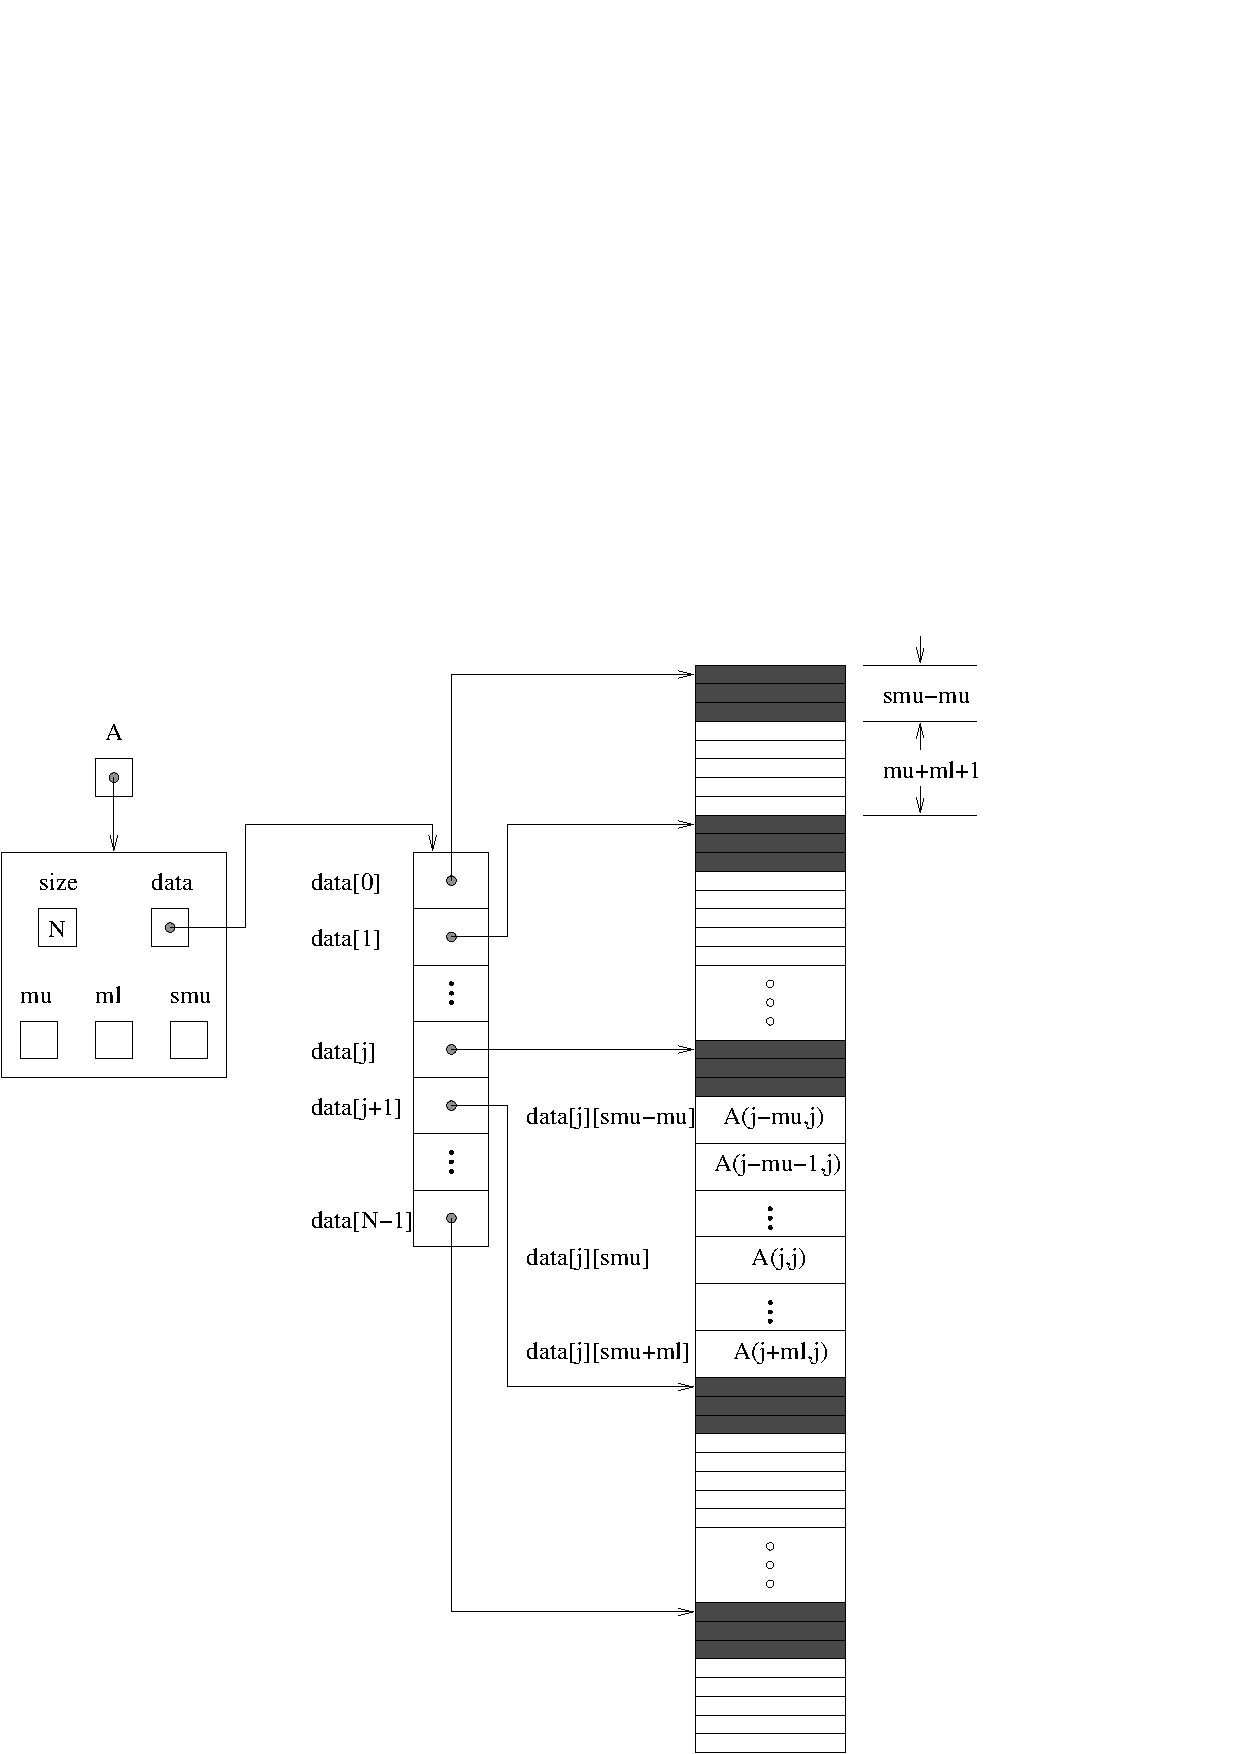
\includegraphics[width=4.5 in]{bandmat}}
\caption[Diagram of the storage for a {\sunmatband} object]
  {Diagram of the storage for the {\sunmatband} module. Here \id{A} is an
  $\id{N} \times \id{N}$ band matrix with upper and lower half-bandwidths \id{mu}
  and \id{ml}, respectively. The rows and columns of \id{A} are
  numbered from $0$ to $\id{N}-1$ and the ($i,j$)-th element of \id{A} is
  denoted \id{A(i,j)}. The greyed out areas of the underlying
  component storage are used by the associated {\sunlinsolband}
  linear solver.}\label{f:sunbandmat}
\end{figure}

\noindent The header file to include when using this module
is \id{sunmatrix/sunmatrix\_band.h}. The {\sunmatband} module
is accessible from all {\sundials} solvers \textit{without}
linking to the \newline
\id{libsundials\_sunmatrixband} module library.


% ====================================================================
\subsection{SUNMatrix\_Band accessor macros}
\label{ss:sunmat_band_macros}
% ====================================================================

The following macros are provided to access the
content of a {\sunmatband} matrix. The prefix \id{SM\_} in the names
denotes that these macros are for \emph{SUNMatrix} implementations,
and the suffix \id{\_B} denotes that these are specific to
the \emph{banded} version.
%%
\begin{itemize}

\item \ID{SM\_CONTENT\_B}

  This routine gives access to the contents of the
  banded \id{SUNMatrix}.

  The assignment \id{A\_cont} $=$ \id{SM\_CONTENT\_B(A)} sets
  \id{A\_cont} to be a pointer to the banded \id{SUNMatrix} content
  structure.

  Implementation:

  \verb|#define SM_CONTENT_B(A)     ( (SUNMatrixContent_Band)(A->content) )|

\item \ID{SM\_ROWS\_B}, \ID{SM\_COLUMNS\_B}, \ID{SM\_UBAND\_B}, \ID{SM\_LBAND\_B}, \ID{SM\_SUBAND\_B}, \ID{SM\_LDIM\_B}, and \ID{SM\_LDATA\_B}

  These macros give individual access to various lengths relevant to the
  content of a banded \id{SUNMatrix}.

  These may be used either to retrieve or to set these values.  For
  example, the assignment \id{A\_rows = SM\_ROWS\_B(A)} sets \id{A\_rows} to be
  the number of rows in the matrix \id{A}.  Similarly, the
  assignment \id{SM\_COLUMNS\_B(A) = A\_cols} sets the number of
  columns in \id{A} to equal \id{A\_cols}.

  Implementation:

  \verb|#define SM_ROWS_B(A)        ( SM_CONTENT_B(A)->M )|

  \verb|#define SM_COLUMNS_B(A)     ( SM_CONTENT_B(A)->N )|

  \verb|#define SM_UBAND_B(A)       ( SM_CONTENT_B(A)->mu )|

  \verb|#define SM_LBAND_B(A)       ( SM_CONTENT_B(A)->ml )|

  \verb|#define SM_SUBAND_B(A)      ( SM_CONTENT_B(A)->s_mu )|

  \verb|#define SM_LDIM_B(A)        ( SM_CONTENT_B(A)->ldim )|

  \verb|#define SM_LDATA_B(A)       ( SM_CONTENT_B(A)->ldata )|

\item \ID{SM\_DATA\_B} and \ID{SM\_COLS\_B}

  These macros give access to the \id{data} and \id{cols} pointers for
  the matrix entries.

  The assignment \id{A\_data = SM\_DATA\_B(A)} sets \id{A\_data} to be
  a pointer to the first component of the data array for the
  banded \id{SUNMatrix} \id{A}.  The assignment \id{SM\_DATA\_B(A) =
  A\_data} sets the data array of \id{A} to be \id{A\_data} by storing
  the pointer \id{A\_data}.

  Similarly, the assignment \id{A\_cols = SM\_COLS\_B(A)} sets \id{A\_cols} to be
  a pointer to the array of column pointers for the banded \id{SUNMatrix} \id{A}.
  The assignment \id{SM\_COLS\_B(A) = A\_cols} sets the column pointer
  array of \id{A} to be \id{A\_cols} by storing the pointer \id{A\_cols}.

  Implementation:

  \verb|#define SM_DATA_B(A)        ( SM_CONTENT_B(A)->data )|

  \verb|#define SM_COLS_B(A)        ( SM_CONTENT_B(A)->cols )|


\item \ID{SM\_COLUMN\_B}, \ID{SM\_COLUMN\_ELEMENT\_B}, and \ID{SM\_ELEMENT\_B}

  These macros give access to the individual columns and entries of
  the data array of a banded \id{SUNMatrix}.

  The assignments \id{SM\_ELEMENT\_B(A,i,j) = a\_ij} and \id{a\_ij =
  SM\_ELEMENT\_B(A,i,j)} reference the (\id{i},\id{j})-th element of the
  $\id{N} \times \id{N}$ band matrix \id{A}, where $0 \le \id{i}, \id{j} \le \id{N}-1$.
  The location (\id{i},\id{j}) should further satisfy
  \id{j}$-$\id{mu} $\le$ \id{i} $\le$ \id{j}$+$\id{ml}.

  The assignment \id{col\_j = SM\_COLUMN\_B(A,j)} sets \id{col\_j} to be
  a pointer to the diagonal element of the \id{j}-th column of the
  $\id{N} \times \id{N}$ band matrix \id{A}, $0 \le \id{j} \le \id{N}-1$.
  The type of the expression \id{SM\_COLUMN\_B(A,j)} is \id{realtype *}.
  The pointer returned by the call \id{SM\_COLUMN\_B(A,j)} can be treated as
  an array which is indexed from $-$\id{mu} to \id{ml}.

  The assignments \id{SM\_COLUMN\_ELEMENT\_B(col\_j,i,j) = a\_ij} and\\
  \id{a\_ij = SM\_COLUMN\_ELEMENT\_B(col\_j,i,j)} reference the
  (\id{i},\id{j})-th entry of the band matrix \id{A} when used in
  conjunction with \id{SM\_COLUMN\_B} to reference the \id{j}-th column
  through \id{col\_j}. The index (\id{i},\id{j}) should satisfy
  \id{j}$-$\id{mu} $\le$ \id{i} $\le$ \id{j}$+$\id{ml}.

  Implementation:

  \verb|#define SM_COLUMN_B(A,j)    ( ((SM_CONTENT_B(A)->cols)[j])+SM_SUBAND_B(A) )|

  \verb|#define SM_COLUMN_ELEMENT_B(col_j,i,j) (col_j[(i)-(j)])|

  \verb|#define SM_ELEMENT_B(A,i,j)|

  \hspace{1in} \verb|( (SM_CONTENT_B(A)->cols)[j][(i)-(j)+SM_SUBAND_B(A)] )|

\end{itemize}


% ====================================================================
\subsection{SUNMatrix\_Band functions}
\label{ss:sunmat_band_functions}
% ====================================================================

The {\sunmatband} module defines banded implementations of all matrix
operations listed in Table \ref{t:sunmatops}. Their names are obtained
from those in Table \ref{t:sunmatops} by appending the
suffix \id{\_Band} (e.g. \id{SUNMatCopy\_Band}).
All the standard matrix operations listed in \ref{t:sunmatops} with the suffix
\id{\_Band} appended are callable via the {\F} 2003 interface by prepending an
`F' (e.g. \id{FSUNMatCopy\_Band}).

The module {\sunmatband} provides the following additional user-callable routines:
%%--------------------------------------
\sunmodfunf{SUNBandMatrix}
{
  This constructor function creates and allocates memory for a banded \id{SUNMatrix}.
  Its arguments are the matrix size, \id{N}, and the upper and lower
  half-bandwidths of the matrix, \id{mu} and \id{ml}.  The stored
  upper bandwidth is set to \id{mu+ml} to accommodate subsequent
  factorization in the {\sunlinsolband} and {\sunlinsollapband} modules.
}
{
  SUNMatrix SUNBandMatrix(sunindextype N, sunindextype mu,
  sunindextype ml)
}
%%--------------------------------------
\sunmodfun{SUNBandMatrixStorage}
{
  This constructor function creates and allocates memory for a banded \id{SUNMatrix}.
  Its arguments are the matrix size, \id{N}, the upper and lower
  half-bandwidths of the matrix, \id{mu} and \id{ml}, and the stored
  upper bandwidth, \id{smu}.  When creating a band \id{SUNMatrix},
  this value should be
  \begin{itemize}
  \item at least min(\id{N}-1,\id{mu}+\id{ml}) if the matrix will be
    used by the {\sunlinsolband} module;
  \item exactly equal to \id{mu}+\id{ml} if the matrix will be used by
    the {\sunlinsollapband} module;
  \item at least \id{mu} if used in some other manner.
  \end{itemize}
  \emph{Note: it is strongly recommended that users call the default
    constructor, \id{SUNBandMatrix}, in all standard use cases.  This
    advanced constructor is used internally within {\sundials}
    solvers, and is provided to users who require banded matrices for
    non-default purposes.}
}
{
  SUNMatrix SUNBandMatrixStorage(sunindextype N, sunindextype mu,
  sunindextype ml, sunindextype smu)
}
%%--------------------------------------
\sunmodfun{SUNBandMatrix\_Print}
{
  This function prints the content of a banded \id{SUNMatrix} to the
  output stream specified by \id{outfile}.  Note: \id{stdout}
  or \id{stderr} may be used as arguments for \id{outfile} to print
  directly to standard output or standard error, respectively.
}
{
  void SUNBandMatrix\_Print(SUNMatrix A, FILE* outfile)
}
%%--------------------------------------
\sunmodfunf{SUNBandMatrix\_Rows}
{
  This function returns the number of rows in the banded \id{SUNMatrix}.
}
{
  sunindextype SUNBandMatrix\_Rows(SUNMatrix A)
}
%%--------------------------------------
\sunmodfunf{SUNBandMatrix\_Columns}
{
  This function returns the number of columns in the banded \id{SUNMatrix}.
}
{
  sunindextype SUNBandMatrix\_Columns(SUNMatrix A)
}
%%--------------------------------------
\sunmodfunf{SUNBandMatrix\_LowerBandwidth}
{
  This function returns the lower half-bandwidth of the banded \id{SUNMatrix}.
}
{
  sunindextype SUNBandMatrix\_LowerBandwidth(SUNMatrix A)
}
%%--------------------------------------
\sunmodfunf{SUNBandMatrix\_UpperBandwidth}
{
  This function returns the upper half-bandwidth of the banded \id{SUNMatrix}.
}
{
  sunindextype SUNBandMatrix\_UpperBandwidth(SUNMatrix A)
}
%%--------------------------------------
\sunmodfunf{SUNBandMatrix\_StoredUpperBandwidth}
{
  This function returns the stored upper half-bandwidth of the banded \id{SUNMatrix}.
}
{
  sunindextype SUNBandMatrix\_StoredUpperBandwidth(SUNMatrix A)
}
%%--------------------------------------
\sunmodfunf{SUNBandMatrix\_LDim}
{
  This function returns the length of the leading dimension of the banded \id{SUNMatrix}.
}
{
  sunindextype SUNBandMatrix\_LDim(SUNMatrix A)
}
%%--------------------------------------
\sunmodfunf{SUNBandMatrix\_Data}
{
  This function returns a pointer to the data array for the banded \id{SUNMatrix}.
}
{
  realtype* SUNBandMatrix\_Data(SUNMatrix A)
}
%%--------------------------------------
\sunmodfun{SUNBandMatrix\_Cols}
{
  This function returns a pointer to the cols array for the banded \id{SUNMatrix}.
}
{
  realtype** SUNBandMatrix\_Cols(SUNMatrix A)
}
%%--------------------------------------
\sunmodfunf{SUNBandMatrix\_Column}
{
  This function returns a pointer to the diagonal entry of the j-th
  column of the banded \id{SUNMatrix}.  The resulting pointer should
  be indexed over the range $-$\id{mu} to \id{ml}.
}
{
  realtype* SUNBandMatrix\_Column(SUNMatrix A, sunindextype j)
}
%%
%%------------------------------------
%%
\paragraph{\bf Notes}

\begin{itemize}

\item
  When looping over the components of a banded \id{SUNMatrix} \id{A},
  the most efficient approaches are to:
  \begin{itemize}
    \item First obtain the component array via \id{A\_data = SM\_DATA\_B(A)} or\\
    \id{A\_data = SUNBandMatrix\_Data(A)} and then
    access \id{A\_data[i]} within the loop.

    \item First obtain the array of column pointers via \id{A\_cols = SM\_COLS\_B(A)} or\\
    \id{A\_cols = SUNBandMatrix\_Cols(A)}, and then
    access \id{A\_cols[j][i]} within the loop.

    \item Within a loop over the columns, access the column pointer via\\
    \id{A\_colj = SUNBandMatrix\_Column(A,j)} and then to access the
    entries within that column using \id{SM\_COLUMN\_ELEMENT\_B(A\_colj,i,j)}.
  \end{itemize}
  All three of these are more efficient than
  using \id{SM\_ELEMENT\_B(A,i,j)} within a double loop.

\item
  {\warn} Within the \id{SUNMatMatvec\_Band} routine, internal
  consistency checks are performed to ensure that the matrix is called
  with consistent {\nvector} implementations.  These are currently
  limited to: {\nvecs}, {\nvecopenmp}, and {\nvecpthreads}.  As additional
  compatible vector implementations are added to {\sundials}, these
  will be included within this compatibility check.

\end{itemize}


% ====================================================================
\subsection{SUNMatrix\_Band Fortran interfaces}
\label{ss:sunmat_band_fortran}
% ====================================================================

The {\sunmatband} module provides a {\F} 2003 module as well as {\F} 77
style interface functions for use from {\F} applications.

\subsubsection*{FORTRAN 2003 interface module}
The \ID{fsunmatrix\_band\_mod} {\F} module defines interfaces to most
{\sunmatband} {\CC} functions using the intrinsic \id{iso\_c\_binding}
module which provides a standardized mechanism for interoperating with {\CC}. As
noted in the {\CC} function descriptions above, the interface functions are
named after the corresponding {\CC} function, but with a leading `F'. For
example, the function \id{SUNBandMatrix} is interfaced as
\id{FSUNBandMatrix}.

The {\F} 2003 {\sunmatband} interface module can be accessed with the \id{use}
statement, i.e. \id{use fsunmatrix\_band\_mod}, and linking to the library
\id{libsundials\_fsunmatrixband\_mod}.{\em lib} in addition to the {\CC} library.
For details on where the library and module file
\id{fsunmatrix\_band\_mod.mod} are installed see Appendix \ref{c:install}.
We note that the module is accessible from the {\F} 2003 {\sundials} integrators
\textit{without} separately linking to the
\id{libsundials\_fsunmatrixband\_mod} library.

\subsubsection*{FORTRAN 77 interface functions}
For solvers that include a {\F} interface module, the {\sunmatband}
module also includes the {\F}-callable
function \id{FSUNBandMatInit(code, N, mu, ml, ier)} to initialize
this {\sunmatband} module for a given {\sundials} solver.
Here \id{code} is an integer input solver id (1 for {\cvode}, 2 for {\ida}, 3
for {\kinsol}, 4 for {\arkode}); \id{N}, \id{mu}, and \id{ml}
are the corresponding band matrix construction arguments (declared
to match C type \id{long int}); and \id{ier} is an error return flag
equal to 0 for success and -1 for failure. Both \id{code} and \id{ier}
are declared to match C type \id{int}. Additionally, when using
{\arkode} with a non-identity mass matrix, the {\F}-callable
function \id{FSUNBandMassMatInit(N, mu, ml, ier)} initializes
this {\sunmatband} module for storing the mass matrix.

%% This is a shared SUNDIALS TEX file with a description of the
%% sparse sunmatrix implementation
%%
\section{The SUNMatrix\_Sparse implementation}\label{ss:sunmat_sparse}

The sparse implementation of the {\sunmatrix} module provided with
{\sundials}, {\sunmatsparse}, is designed to work with either
\emph{compressed-sparse-column} (CSC) or \emph{compressed-sparse-row}
(CSR) sparse matrix formats.  To this end, it defines the {\em
content} field of \id{SUNMatrix} to be the following structure:
%%
\begin{verbatim} 
struct _SUNMatrixContent_Sparse {
  sunindextype M;
  sunindextype N;
  sunindextype NNZ;
  sunindextype NP;
  realtype *data;
  int sparsetype;
  sunindextype *indexvals;
  sunindextype *indexptrs;
  /* CSC indices */
  sunindextype **rowvals;
  sunindextype **colptrs;
  /* CSR indices */
  sunindextype **colvals;
  sunindextype **rowptrs;
};
\end{verbatim}
%%
A diagram of the underlying data representation for a
CSC matrix is shown in Figure \ref{f:sparsemat} (the CSR format is
similar).  A more complete description of the parts of
this \emph{content} field is given below: 
\begin{args}[sparsetype]
  \item[M]  - number of rows
  \item[N]  - number of columns
  \item[NNZ]  - maximum number of nonzero entries in the matrix
    (allocated length of \id{data} and \id{indexvals} arrays)
  \item[NP]  - number of index pointers (e.g. number of column pointers for 
    CSC matrix). For CSC matrices $\id{NP}=\id{N}$, and for CSR
    matrices $\id{NP}=\id{M}$. This value is set automatically based
    the input for \verb|sparsetype|.
  \item[data]  - pointer to a contiguous block of \id{realtype}
    variables (of length \id{NNZ}), containing the values of the
    nonzero entries in the matrix
  \item[sparsetype]  - type of the sparse matrix (\id{CSC\_MAT} or \id{CSR\_MAT})
  \item[indexvals] - pointer to a contiguous block of \id{int} variables
    (of length \id{NNZ}), containing the row indices (if CSC) or column
   indices (if CSR) of each nonzero matrix entry held in \id{data}
  \item[indexptrs]  - pointer to a contiguous block of \id{int}
    variables (of length \id{NP+1}). For CSC matrices each 
    entry provides the index of the first column entry into the 
    \id{data} and \id{indexvals} arrays, e.g. if \id{indexptr[3]=7}, then 
    the first nonzero entry in the fourth column of the matrix is 
    located in \id{data[7]}, and is located in row \id{indexvals[7]} of the 
    matrix.  The last entry contains the total number of nonzero values in 
    the matrix and hence points one past the end of the active data in the 
    \id{data} and \id{indexvals} arrays. For CSR matrices, each entry provides 
    the index of the first row entry into the \id{data} and \id{indexvals} 
    arrays.
\end{args}
\noindent The following pointers are added to the \id{SlsMat} type for
  user convenience, to provide a more intuitive interface to the CSC
  and CSR sparse matrix data structures. They are set automatically
  when creating a sparse {\sunmatrix}, based on the sparse matrix storage
  type.  
\begin{args}[colptrs]
  \item[rowvals] - pointer to \verb|indexvals| when \id{sparsetype} is \id{CSC\_MAT},
    otherwise set to \verb|NULL|.
  \item[colptrs] - pointer to \verb|indexptrs| when \id{sparsetype} is \id{CSC\_MAT},
    otherwise set to \verb|NULL|.
  \item[colvals] - pointer to \verb|indexvals| when \id{sparsetype} is \id{CSR\_MAT},
    otherwise set to \verb|NULL|.
  \item[rowptrs] - pointer to \verb|indexptrs| when \id{sparsetype} is \id{CSR\_MAT},
    otherwise set to \verb|NULL|.
\end{args}
For example, the $5\times 4$ CSC matrix
\[
  \left[\begin{array}{cccc} 
     0 & 3 & 1 & 0\\
     3 & 0 & 0 & 2\\
     0 & 7 & 0 & 0\\
     1 & 0 & 0 & 9\\
     0 & 0 & 0 & 5
  \end{array}\right]
\]
could be stored in this structure as either
\begin{verbatim}
  M = 5;
  N = 4;
  NNZ = 8;
  NP = N;
  data = {3.0, 1.0, 3.0, 7.0, 1.0, 2.0, 9.0, 5.0};
  sparsetype = CSC_MAT;
  indexvals = {1, 3, 0, 2, 0, 1, 3, 4};
  indexptrs = {0, 2, 4, 5, 8};
\end{verbatim}
or 
\begin{verbatim}
  M = 5;
  N = 4;
  NNZ = 10;
  NP = N;
  data = {3.0, 1.0, 3.0, 7.0, 1.0, 2.0, 9.0, 5.0, *, *};
  sparsetype = CSC_MAT;
  indexvals = {1, 3, 0, 2, 0, 1, 3, 4, *, *};
  indexptrs = {0, 2, 4, 5, 8};
\end{verbatim}
where the first has no unused space, and the second has additional
storage (the entries marked with \texttt{*} may contain any values).
Note in both cases that the final value in \id{indexptrs} is $8$,
indicating the total number of nonzero entries in the matrix.

Similarly, in CSR format, the same matrix could be stored as
\begin{verbatim}
  M = 5;
  N = 4;
  NNZ = 8;
  NP = M;
  data = {3.0, 1.0, 3.0, 2.0, 7.0, 1.0, 9.0, 5.0};
  sparsetype = CSR_MAT;
  indexvals = {1, 2, 0, 3, 1, 0, 3, 3};
  indexptrs = {0, 2, 4, 5, 7, 8};
\end{verbatim}

%%
%%--------------------------------------------
%%
\begin{figure}
\centerline{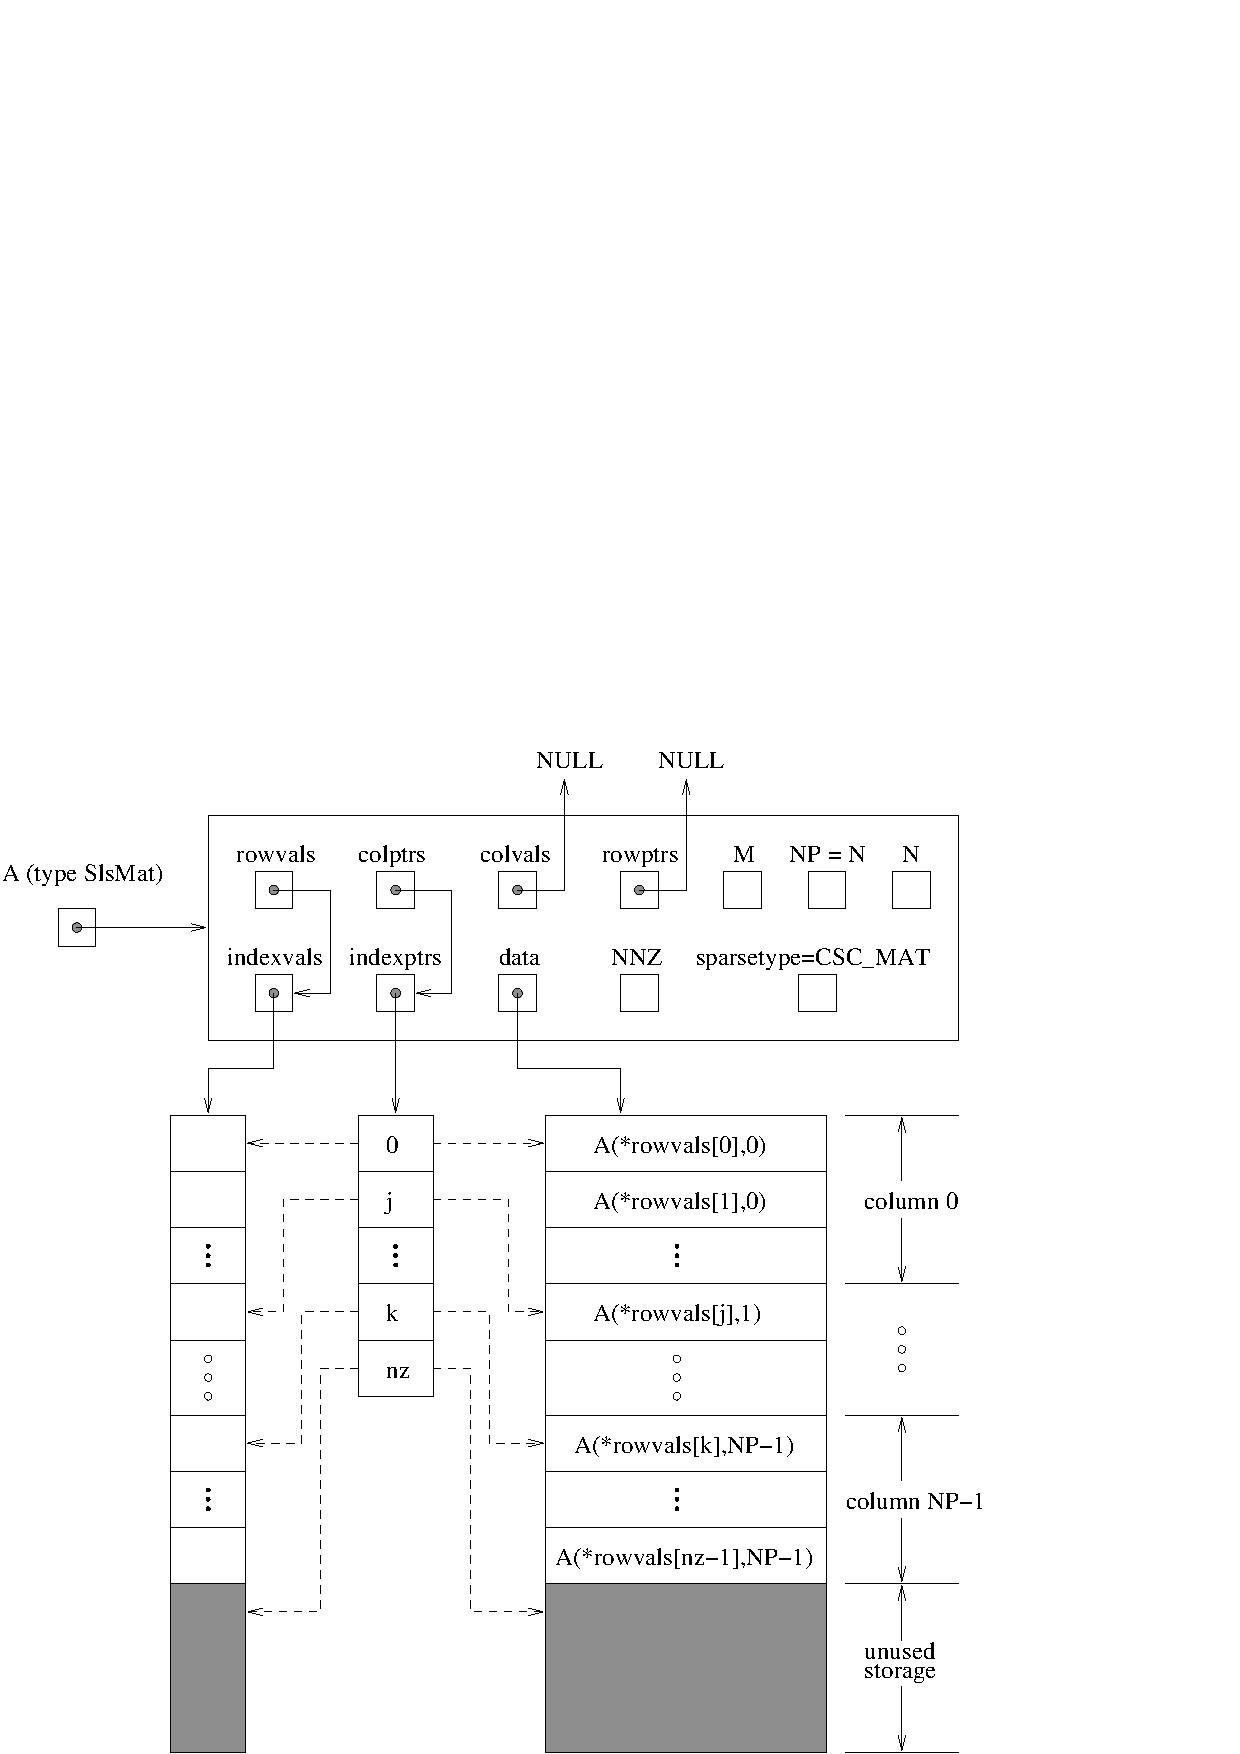
\includegraphics[width=4.5 in]{cscmat}}
\caption[Diagram of the storage for a compressed-sparse-column matrix] 
  {Diagram of the storage for a compressed-sparse-column
  matrix. Here \id{A} is an $\id{M} \times \id{N}$ sparse matrix with storage
  for up to \id{NNZ} nonzero entries (the allocated length of
  both \id{data} and \id{indexvals}).  The entries in \id{indexvals}
  may assume values from $0$ to $\id{M}-1$, corresponding to the row index
  (zero-based) of each nonzero value.  The entries in \id{data} contain
  the values of the nonzero entries, with the row $i$, column $j$
  entry of \id{A} (again, zero-based) denoted as \id{A(i,j)}.
  The \id{indexptrs} array contains $\id{N}+1$ entries; the first $\id{N}$
  denote the starting index of each column within the \id{indexvals}
  and \id{data} arrays, while the final entry points one past the
  final nonzero entry.  Here, although \id{NNZ} values are allocated,
  only \id{nz} are actually filled in; the greyed-out portions
  of \id{data} and \id{indexvals} indicate extra allocated
  space.}\label{f:sparsemat} 
\end{figure}

\noindent The header file to include when using this module 
is \id{sunmatrix/sunmatrix\_sparse.h}. The {\sunmatsparse} module
is accessible from all {\sundials} solvers \textit{without}
linking to the \\
\id{libsundials\_sunmatrixsparse} module library.


% ====================================================================
\subsection{SUNMatrix\_Sparse accessor macros}
\label{ss:sunmat_sparse_macros}
% ====================================================================

The following macros are provided to access the
content of a {\sunmatsparse} matrix. The prefix \id{SM\_} in the names
denotes that these macros are for \emph{SUNMatrix} implementations,
and the suffix \id{\_S} denotes that these are specific to
the \emph{sparse} version.
%%
\begin{itemize}

\item \ID{SM\_CONTENT\_S}
    
  This routine gives access to the contents of the
  sparse \id{SUNMatrix}.
  
  The assignment \id{A\_cont} $=$ \id{SM\_CONTENT\_S(A)} sets           
  \id{A\_cont} to be a pointer to the sparse \id{SUNMatrix} content  
  structure.                                             
                                                            
  Implementation: 
  
  \verb|#define SM_CONTENT_S(A)     ( (SUNMatrixContent_Sparse)(A->content) )|
  
\item \ID{SM\_ROWS\_S}, \ID{SM\_COLUMNS\_S}, \ID{SM\_NNZ\_S}, \ID{SM\_NP\_S}, and \ID{SM\_SPARSETYPE\_S}

  These macros give individual access to various lengths relevant to the
  content of a sparse \id{SUNMatrix}.
                                                               
  These may be used either to retrieve or to set these values.  For
  example, the assignment \id{A\_rows = SM\_ROWS\_S(A)} sets \id{A\_rows} to be
  the number of rows in the matrix \id{A}.  Similarly, the
  assignment \id{SM\_COLUMNS\_S(A) = A\_cols} sets the number of
  columns in \id{A} to equal \id{A\_cols}.
  
  Implementation: 
  
  \verb|#define SM_ROWS_S(A)        ( SM_CONTENT_S(A)->M )|

  \verb|#define SM_COLUMNS_S(A)     ( SM_CONTENT_S(A)->N )|

  \verb|#define SM_NNZ_S(A)         ( SM_CONTENT_S(A)->NNZ )|

  \verb|#define SM_NP_S(A)          ( SM_CONTENT_S(A)->NP )|

  \verb|#define SM_SPARSETYPE_S(A)  ( SM_CONTENT_S(A)->sparsetype )|


\item \ID{SM\_DATA\_S}, \ID{SM\_INDEXVALS\_S}, and \ID{SM\_INDEXPTRS\_S}
                                                            
  These macros give access to the \id{data} and index arrays for
  the matrix entries.

  The assignment \id{A\_data = SM\_DATA\_S(A)} sets \id{A\_data} to be     
  a pointer to the first component of the data array for the
  sparse \id{SUNMatrix} \id{A}.  The assignment \id{SM\_DATA\_S(A) =
  A\_data} sets the data array of \id{A} to be \id{A\_data} by storing
  the pointer \id{A\_data}. 
  
  Similarly, the assignment \id{A\_indexvals = SM\_INDEXVALS\_S(A)}
  sets \id{A\_indexvals} to be a pointer to the array of index values
  (i.e.~row indices for a CSC matrix, or column indices for a CSR
  matrix) for the sparse \id{SUNMatrix} \id{A}.  The
  assignment \id{A\_indexptrs = SM\_INDEXPTRS\_S(A)}
  sets \id{A\_indexptrs} to be a pointer to the array of index
  pointers (i.e.~the starting indices in the data/indexvals arrays for
  each row or column in CSR or CSC formats, respectively).
  
  Implementation:

  \verb|#define SM_DATA_S(A)        ( SM_CONTENT_S(A)->data )|

  \verb|#define SM_INDEXVALS_S(A)   ( SM_CONTENT_S(A)->indexvals )|

  \verb|#define SM_INDEXPTRS_S(A)   ( SM_CONTENT_S(A)->indexptrs )|

\end{itemize}


% ====================================================================
\subsection{SUNMatrix\_Sparse functions}
\label{ss:sunmat_sparse_functions}
% ====================================================================

The {\sunmatsparse} module defines sparse implementations of all matrix
operations listed in Section \ref{ss:sunmatrix_functions}. Their names are obtained
from those in Section \ref{ss:sunmatrix_functions} by appending the
suffix \id{\_Sparse} (e.g. \id{SUNMatCopy\_Sparse}). 
All the standard matrix operations listed in Section \ref{ss:sunmatrix_functions} with the suffix
\id{\_Sparse} appended are callable via the {\F} 2003 interface by prepending an
`F' (e.g. \id{FSUNMatCopy\_Sparse}).

The module {\sunmatsparse} provides the following additional
user-callable routines: 
%%--------------------------------------
\sunmodfunf{SUNSparseMatrix}
{
  This function creates and allocates memory for a sparse \id{SUNMatrix}.
  Its arguments are the number of rows and columns of the
  matrix, \id{M} and \id{N}, the maximum number of nonzeros to be
  stored in the matrix, \id{NNZ}, and a flag \id{sparsetype}
  indicating whether to use CSR or CSC format (valid arguments
  are \id{CSR\_MAT} or \id{CSC\_MAT}). 
}
{
  SUNMatrix SUNSparseMatrix(sunindextype M, sunindextype N,
  \newlinefill{SUNMatrix SUNSparseMatrix}
  sunindextype NNZ, int sparsetype)
}
%%--------------------------------------
\sunmodfunf{SUNSparseFromDenseMatrix}
{
  This function creates a new sparse matrix from an existing dense
  matrix by copying all values with magnitude larger than \id{droptol}
  into the sparse matrix structure.

  Requirements:
  \begin{itemize}
  \item \id{A} must have type \id{SUNMATRIX\_DENSE};
  \item \id{droptol} must be non-negative;
  \item \id{sparsetype} must be either \id{CSC\_MAT} or \id{CSR\_MAT}.
  \end{itemize}
  The function returns NULL if any requirements are violated, or if
  the matrix storage request cannot be satisfied. 
}
{
  SUNMatrix SUNSparseFromDenseMatrix(SUNMatrix A, realtype droptol,
  \newlinefill{SUNMatrix SUNSparseFromDenseMatrix}
  int sparsetype);
}
%%--------------------------------------
\sunmodfunf{SUNSparseFromBandMatrix}
{
  This function creates a new sparse matrix from an existing band
  matrix by copying all values with magnitude larger than \id{droptol}
  into the sparse matrix structure.

  Requirements:
  \begin{itemize}
  \item \id{A} must have type \id{SUNMATRIX\_BAND};
  \item \id{droptol} must be non-negative;
  \item \id{sparsetype} must be either \id{CSC\_MAT} or \id{CSR\_MAT}.
  \end{itemize}
  The function returns NULL if any requirements are violated, or if
  the matrix storage request cannot be satisfied. 
}
{
  SUNMatrix SUNSparseFromBandMatrix(SUNMatrix A, realtype droptol,
  \newlinefill{SUNMatrix SUNSparseFromBandMatrix}
  int sparsetype);
}
%%--------------------------------------
\sunmodfunf{SUNSparseMatrix\_Realloc}
{
  This function reallocates internal storage arrays in a sparse matrix
  so that the resulting sparse matrix has no wasted space (i.e.~the
  space allocated for nonzero entries equals the actual number of
  nonzeros, \id{indexptrs[NP]}). Returns 0 on success and 
  1 on failure (e.g.~if the input matrix is not sparse).
}
{
  int SUNSparseMatrix\_Realloc(SUNMatrix A)
}
%%--------------------------------------
\sunmodfunf{SUNSparseMatrix\_Reallocate}
{
  This function reallocates internal storage arrays in a sparse matrix
  so that the resulting sparse matrix has storage for a specified
  number of nonzeros. Returns 0 on success and 
  1 on failure (e.g.~if the input matrix is not sparse or if NNZ is
  negative). 
}
{
  int SUNSparseMatrix\_Reallocate(SUNMatrix A, sunindextype NNZ)
}
%%--------------------------------------
\sunmodfun{SUNSparseMatrix\_Print}
{
  This function prints the content of a sparse \id{SUNMatrix} to the
  output stream specified by \id{outfile}.  Note: \id{stdout}
  or \id{stderr} may be used as arguments for \id{outfile} to print
  directly to standard output or standard error, respectively.
}
{
  void SUNSparseMatrix\_Print(SUNMatrix A, FILE* outfile)
}
%%--------------------------------------
\sunmodfunf{SUNSparseMatrix\_Rows}
{
  This function returns the number of rows in the sparse \id{SUNMatrix}.
}
{
  sunindextype SUNSparseMatrix\_Rows(SUNMatrix A)
}
%%--------------------------------------
\sunmodfunf{SUNSparseMatrix\_Columns}
{
  This function returns the number of columns in the sparse \id{SUNMatrix}.
}
{
  sunindextype SUNSparseMatrix\_Columns(SUNMatrix A)
}
%%--------------------------------------
\sunmodfunf{SUNSparseMatrix\_NNZ}
{
  This function returns the number of entries allocated for nonzero
  storage for  the sparse matrix \id{SUNMatrix}.
}
{
  sunindextype SUNSparseMatrix\_NNZ(SUNMatrix A)
}
%%--------------------------------------
\sunmodfunf{SUNSparseMatrix\_NP}
{
  This function returns the number of columns/rows for the
  sparse \id{SUNMatrix}, depending on whether the matrix uses CSC/CSR
  format, respectively.  The \id{indexptrs} array has \id{NP+1} entries.
}
{
  sunindextype SUNSparseMatrix\_NP(SUNMatrix A)
}
%%--------------------------------------
\sunmodfunf{SUNSparseMatrix\_SparseType}
{
  This function returns the storage type (\id{CSR\_MAT}
  or \id{CSC\_MAT}) for the sparse \id{SUNMatrix}.
}
{
  int SUNSparseMatrix\_SparseType(SUNMatrix A)
}
%%--------------------------------------
\sunmodfunf{SUNSparseMatrix\_Data}
{
  This function returns a pointer to the data array for the
  sparse \id{SUNMatrix}. 
}
{
  realtype* SUNSparseMatrix\_Data(SUNMatrix A)
}
%%--------------------------------------
\sunmodfunf{SUNSparseMatrix\_IndexValues}
{
  This function returns a pointer to index value array for the sparse
  \id{SUNMatrix}: for CSR format this is the column index for each nonzero
  entry, for CSC format this is the row index for each nonzero entry.
}
{
  sunindextype* SUNSparseMatrix\_IndexValues(SUNMatrix A)
}
%%--------------------------------------
\sunmodfunf{SUNSparseMatrix\_IndexPointers}
{
  This function returns a pointer to the index pointer array for the
  sparse \id{SUNMatrix}: for CSR format this is the location of the first
  entry of each row in the \id{data} and \id{indexvalues} arrays, for
  CSC format this is the location of the first entry of each column.
}
{
  sunindextype* SUNSparseMatrix\_IndexPointers(SUNMatrix A)
}
%%
%%------------------------------------
%%
{\warn} Within the \id{SUNMatMatvec\_Sparse} routine, internal
consistency checks are performed to ensure that the matrix is called
with consistent {\nvector} implementations.  These are currently
limited to: {\nvecs}, {\nvecopenmp}, {\nvecpthreads}, and {\nveccuda}
when using managed memory.  As additional compatible vector implementations
are added to {\sundials}, these will be included within this compatibility check. 


% ====================================================================
\subsection{SUNMatrix\_Sparse Fortran interfaces}
\label{ss:sunmat_sparse_fortran}
% ====================================================================

The {\sunmatsparse} module provides a {\F} 2003 module as well as {\F} 77
style interface functions for use from {\F} applications.

\subsubsection*{FORTRAN 2003 interface module}
The \ID{fsunmatrix\_sparse\_mod} {\F} module defines interfaces to most
{\sunmatsparse} {\CC} functions using the intrinsic \id{iso\_c\_binding}
module which provides a standardized mechanism for interoperating with {\CC}. As
noted in the {\CC} function descriptions above, the interface functions are
named after the corresponding {\CC} function, but with a leading `F'. For
example, the function \id{SUNSparseMatrix} is interfaced as
\id{FSUNSparseMatrix}.

The {\F} 2003 {\sunmatsparse} interface module can be accessed with the \id{use}
statement, i.e. \id{use fsunmatrix\_sparse\_mod}, and linking to the library
\id{libsundials\_fsunmatrixsparse\_mod}.{\em lib} in addition to the {\CC} library.
For details on where the library and module file
\id{fsunmatrix\_sparse\_mod.mod} are installed see Appendix \ref{c:install}.
We note that the module is accessible from the {\F} 2003 {\sundials} integrators
\textit{without} separately linking to the
\id{libsundials\_fsunmatrixsparse\_mod} library.

\subsubsection*{FORTRAN 77 interface functions}
For solvers that include a Fortran interface module, the {\sunmatsparse}
module also includes the Fortran-callable
function \id{FSUNSparseMatInit(code, M, N, NNZ, sparsetype, ier)} to
initialize this {\sunmatsparse} module for a given {\sundials} solver.
Here \id{code} is an integer input for the solver id (1 for {\cvode},
2 for {\ida}, 3 for {\kinsol}, 4 for {\arkode}); \id{M}, \id{N}
and \id{NNZ} are the corresponding sparse matrix construction
arguments (declared to match C type \id{long
int}); \id{sparsetype} is an integer flag indicating the sparse
storage type (0 for CSC, 1 for CSR); and \id{ier} is an error return
flag equal to 0 for success and -1 for failure. Each of \id{code},
\id{sparsetype} and \id{ier} are declared so as to match C
type \id{int}. Additionally, when using {\arkode} with a non-identity
mass matrix, the Fortran-callable
function \id{FSUNSparseMassMatInit(M, N, NNZ, sparsetype, ier)} 
initializes this {\sunmatsparse} module for storing the mass matrix.

%% This is a shared SUNDIALS TEX file with a description of the
%% SuperLU_DIST SLUNRloc SUNMatrix implementation
%%
\section{The SUNMatrix\_SLUNRloc implementation}\label{ss:sunmat_slunrloc}

The {\sunmatslunrloc} implementation of the {\sunmatrix} module provided with
{\sundials} is an adapter for the \id{SuperMatrix} structure provided by the
{\superludist} sparse matrix factorization and solver library written by
X. Sherry Li \cite{SuperLUDIST_site,GDL:07,LD:03,SLUUG:99}.
It is designed to be used with the {\sunlinsolsludist} linear solver
discussed in Section~\ref{ss:sunlinsol_sludist}. To this end, it defines the
{\em content} field of \id{SUNMatrix} to be the following structure:
%%
\begin{verbatim}
struct _SUNMatrixContent_SLUNRloc {
  booleantype   own_data;
  gridinfo_t    *grid;
  sunindextype  *row_to_proc;
  pdgsmv_comm_t *gsmv_comm;
  SuperMatrix   *A_super;
  SuperMatrix   *ACS_super;
};
\end{verbatim}
%%

A more complete description of the this \emph{content} field is given below:

\begin{description}
  \item[own\_data] - a flag which indicates if the SUNMatrix is responsible for freeing
    \id{A\_super}
  \item[grid] - pointer to the {\superludist} structure that stores the 2D process grid
  \item[row\_to\_proc] - a mapping between the rows in the matrix and the process it
    resides on; will be \id{NULL} until the \id{SUNMatMatvecSetup} routine is called
  \item[gsmv\_comm] - pointer to the {\superludist} structure that stores the
    communication information needed for matrix-vector multiplication; will be
    \id{NULL} until the \id{SUNMatMatvecSetup} routine is called
  \item[A\_super] - pointer to the underlying {\superludist} \id{SuperMatrix} with
      \id{Stype = SLU\_NR\_loc, Dtype = SLU\_D, Mtype = SLU\_GE}; must have the
      full diagonal present to be used with \id{SUNMatScaleAddI} routine
  \item[ACS\_super] - a column-sorted version of the matrix needed to perform matrix-vector
    multiplication; will be \id{NULL} until the routine \id{SUNMatMatvecSetup}
    routine is called
\end{description}

\noindent The header file to include when using this module
is \id{sunmatrix/sunmatrix\_slunrloc.h}. The installed module
library to link to is \id{libsundials\_sunmatrixslunrloc.\textit{lib}}
where \id{\em.lib} is typically \id{.so} for shared libraries and
\id{.a} for static libraries.


% ====================================================================
\subsection{SUNMatrix\_SLUNRloc functions}
\label{ss:sunmat_slunrloc_functions}
% ====================================================================

The module {\sunmatslunrloc} provides the following user-callable routines:
%%--------------------------------------
%%
\ucfunction{SUNMatrix\_SLUNRloc}
{
  A = SUNMatrix\_SLUNRloc(Asuper, grid);
}
{
  The function \ID{SUNMatrix\_SLUNRloc} creates and allocates memory for a
  {\sunmatslunrloc} object.
}
{
  \begin{args}
  \item[Asuper] (\id{SuperMatrix*})
      a fully-allocated {\superludist} \id{SuperMatrix} that the SUNMatrix will
      wrap; must have \id{Stype = SLU\_NR\_loc, Dtype = SLU\_D, Mtype = SLU\_GE}
      to be compatible
  \item[grid] (\id{gridinfo\_t*}) the initialized {\superludist} 2D process grid structure
  \end{args}
}
{
  a \id{SUNMatrix} object if \id{Asuper} is compatible else \id{NULL}
}
{
}

\ucfunction{SUNMatrix\_SLUNRloc\_Print}
{
  SUNMatrix\_SLUNRloc\_Print(A, fp);
}
{
  The function \ID{SUNMatrix\_SLUNRloc\_Print} prints the underlying
  \id{SuperMatrix} content.
}
{
  \begin{args}
  \item[A] (\id{SUNMatrix}) the matrix to print
  \item[fp] (\id{FILE}) the file pointer used for printing
  \end{args}
}
{
  \id{void}
}
{
}

\ucfunction{SUNMatrix\_SLUNRloc\_SuperMatrix}
{
  Asuper = SUNMatrix\_SLUNRloc\_SuperMatrix(A);
}
{
  The function \ID{SUNMatrix\_SLUNRloc\_SuperMatrix} provides access
  to the underlying {\superludist} \id{SuperMatrix} of \id{A}.
}
{
  \begin{args}
  \item[A] (\id{SUNMatrix}) the matrix to access
  \end{args}
}
{
  \id{SuperMatrix*}
}
{
}

\ucfunction{SUNMatrix\_SLUNRloc\_ProcessGrid}
{
  grid = SUNMatrix\_SLUNRloc\_ProcessGrid(A);
}
{
  The function \ID{SUNMatrix\_SLUNRloc\_ProcessGrid} provides access
  to the {\superludist} \id{gridinfo\_t} structure associated with \id{A}.
}
{
  \begin{args}
  \item[A] (\id{SUNMatrix}) the matrix to access
  \end{args}
}
{
  \id{gridinfo\_t*}
}
{
}

\ucfunction{SUNMatrix\_SLUNRloc\_OwnData}
{
  does\_own\_data = SUNMatrix\_SLUNRloc\_OwnData(A);
}
{
  The function \ID{SUNMatrix\_SLUNRloc\_OwnData} returns true if the \id{SUNMatrix}
  object is responsible for freeing \id{A\_super}, otherwise it returns false.
}
{
  \begin{args}
  \item[A] (\id{SUNMatrix}) the matrix to access
  \end{args}
}
{
  \id{booleantype}
}
{
}

The {\sunmatslunrloc} module defines implementations of all generic \id{SUNMatrix} operations
listed in Table \ref{t:sunmatops}:

\begin{itemize}
  \item \id{SUNMatGetID\_SLUNRloc} - returns \id{SUNMATRIX\_SLUNRLOC}
  \item \id{SUNMatClone\_SLUNRloc}
  \item \id{SUNMatDestroy\_SLUNRloc}
  \item \id{SUNMatSpace\_SLUNRloc} - this only returns information for the storage within the
    matrix interface, i.e. storage for \id{row\_to\_proc}
  \item \id{SUNMatZero\_SLUNRloc}
  \item \id{SUNMatCopy\_SLUNRloc}
  \item \id{SUNMatScaleAdd\_SLUNRloc} - performs $A = cA + B$, but $A$ and $B$ must have the same sparsity pattern 
  \item \id{SUNMatScaleAddI\_SLUNRloc} - performs $A = cA + I$, but the diagonal of $A$ must be present
  \item \id{SUNMatMatvecSetup\_SLUNRloc} - initializes the {\superludist} parallel communication
    structures needed to perform a matrix-vector product; only needs to be called before the
    first call to \id{SUNMatMatvec} or if the matrix changed since the last setup
  \item \id{SUNMatMatvec\_SLUNRloc}
\end{itemize}

%%------------------------------------
%%
{\warn} The {\sunmatslunrloc} module requires that the complete diagonal, i.e. nonzeros and zeros,
is present in order to use the \id{SUNMatScaleAddI} operation.

% % ====================================================================
% \subsection{SUNMatrix\_SLUNRloc Fortran interfaces}
% \label{ss:sunmat_slunrloc_fortran}
% % ====================================================================

% The {\sunmatslunrloc} module provides a {\F} 2003 module as well as {\F} 77
% style interface functions for use from {\F} applications.

% \subsubsection*{FORTRAN 2003 interface module}
% The \ID{fsunmatrix\_slunrloc\_mod} {\F} module defines interfaces to most
% {\sunmatslunrloc} {\CC} functions using the intrinsic \id{iso\_c\_binding}
% module which provides a standardized mechanism for interoperating with {\CC}. As
% noted in the {\CC} function descriptions above, the interface functions are
% named after the corresponding {\CC} function, but with a leading `F'. For
% example, the function \id{SUNMatrix\_SLUNRloc} is interfaced as
% \id{FSUNMatrix\_SLUNRloc}.

% The {\F} 2003 {\sunmatslunrloc} interface module can be accessed with the \id{use}
% statement, i.e. \id{use fsunmatrix\_slunrloc\_mod}, and linking to the library
% \id{libsundials\_fsunmatrixslunrloc\_mod}.{\em lib} in addition to the {\CC} library.
% For details on where the library and module file \id{fsunmatrix\_slunrloc\_mod.mod}
% are installed see Appendix \ref{c:install}.


%% This is a shared SUNDIALS TEX file with a description of the
%% cuSPARSE SUNMatrix implementation.
%%
\section{The SUNMatrix\_cuSparse implementation}\label{ss:sunmat_cusparse}

The \id{SUNMATRIX\_CUSPARSE} implementation of the \id{SUNMatrix} module provided with
{\sundials}, is an interface to the NVIDIA cuSPARSE matrix for use on NVIDIA GPUs
\cite{cuSPARSE}. All data stored by this matrix implementation resides on the
GPU at all times. The implementation currently supports the cuSPARSE CSR matrix
format described in the cuSPARSE documentation as well as a unique low-storage
format for block-diagonal matrices of the form
\begin{equation*}
  \mathbf{A} =
  \begin{bmatrix}
    \mathbf{A_1} & 0 & \cdots & 0\\
    0 & \mathbf{A_2} & \cdots & 0\\
    \vdots & \vdots & \ddots & \vdots\\
    0 & 0 & \cdots & \mathbf{A_n}\\
  \end{bmatrix}
\end{equation*}
where all the block matrices $A_j$ share the same sparsity pattern.
We will refer to this format as BCSR (not to be confused with the canonical BSR format where
each block is stored as dense). In this format, the CSR column indices and row pointers
are only stored for the first block and are computed only as necessary for other blocks.
This can drastically reduce the amount of storage required compared to the regular CSR
format when there is a large number of blocks. This format is well-suited for, and
intended to be used with the \ref{ss:sunlinsol_cuspbqr}.

\noindent The header file to include when using this module is
\id{sunmatrix/sunmatrix\_cusparse.h}. The installed library to link to is
\id{libsundials\_sunmatrixcusparse.\textit{lib}} where \id{\em.lib} is typically \id{.so}
for shared libraries and \id{.a} for static libraries.
\newline
\newline
{\warn}The \id{SUNMatrix\_cuSparse} module is experimental and subject to change.

% ====================================================================
\subsection{SUNMatrix\_cuSparse functions}
\label{ss:sunmat_cusparse_functions}
% ====================================================================

The \id{SUNMATRIX\_CUSPARSE} module defines GPU-enabled sparse implementations of all matrix
operations listed in the section :ref:`SUNMatrix.Ops` except for the ``SUNMatSpace``
and ``SUNMatMatvecSetup`` operations:

\begin{enumerate}
  \item \id{SUNMatGetID\_cuSparse} -- returns \id{SUNMATRIX\_CUSPARSE}
  \item \id{SUNMatClone\_cuSparse}
  \item \id{SUNMatDestroy\_cuSparse}
  \item \id{SUNMatZero\_cuSparse}
  \item \id{SUNMatCopy\_cuSparse}
  \item \id{SUNMatScaleAdd\_cuSparse} -- performs $A = cA + B$, where $A$ and $B$
    must have the same sparsity pattern
  \item \id{SUNMatScaleAddI\_cuSparse} -- performs $A = cA + I$, where the diagonal
    of $A$ must be present
  \item \id{SUNMatMatvec\_cuSparse}
\end{enumerate}


In addition, the SUNMATRIX\_CUSPARSE module defines the following implementation specific
functions:

%%--------------------------------------
%%
\ucfunction{SUNMatrix\_cuSparse\_NewCSR}
{
  A = SUNMatrix\_cuSparse\_NewCSR(M, N, NNZ, cusp)
}
{
  This constructor function creates and allocates memory for a \id{SUMATRIX\_CUSPARSE}
  \id{SUNMatrix} that uses the CSR storage format.
}
{
  \begin{args}
  \item[M] (\id{int}) the number of matrix rows
  \item[N] (\id{int}) the number of matrix columns
  \item[NNZ] (\id{int}) the number of matrix nonzeros
  \item[cusp] (\id{cusparseHandle\_t}) a valid \id{cusparseHandle\_t}
  \end{args}
}
{
  a \id{SUNMatrix} object if successful else \id{NULL}
}
{
}

%%--------------------------------------
%%
\ucfunction{SUNMatrix\_cuSparse\_NewBlockCSR}
{
  A = SUNMatrix\_cuSparse\_NewBlockCSR(nblocks, blockrows, blockcols, blocknnz, cusp)
}
{
  This constructor function creates and allocates memory for a \id{SUMATRIX\_CUSPARSE}
  \id{SUNMatrix} that leverages the \id{SUNMAT\_CUSPARSE\_BCSR} storage
  format to store a block diagonal matrix where each block shares the same
  sparsity pattern. \textbf{The blocks must be square.}
}
{
  \begin{args}
  \item[nblocks] (\id{int}) the number of matrix blocks
  \item[blockrows] (\id{int}) the number of rows for a block
  \item[blockcols] (\id{int}) the number of columns for a block
  \item[blocknnz] (\id{int}) the number of nonzeros in a block
  \item[cusp] a valid \id{cusparseHandle\_t}
  \end{args}
}
{
  a \id{SUNMatrix} object if successful else \id{NULL}
}
{
  The \id{SUNMAT\_CUSPARSE\_BCSR} format currently only supports square matrices.
}

%%--------------------------------------
%%
\ucfunction{SUNMatrix\_cuSparse\_MakeCSR}
{
  A = SUNMatrix\_cuSparse\_MakeCSR(mat\_descr, M, N, NNZ, rowptrs, colind, data, cusp)
}
{
  This constructor function creates and allocates memory for a \id{SUMATRIX\_CUSPARSE}
  \id{SUNMatrix} that uses the CSR storage format from the user provided pointers.
}
{
  \begin{args}
  \item[mat\_decsr] a valid \id{cusparseMatDescr\_t} object;
    must use \id{CUSPARSE\_INDEX\_BASE\_ZERO} indexing
  \item[M] (\id{int}) the number of matrix rows
  \item[N] (\id{int}) the number of matrix columns
  \item[NNZ] (\id{int}) the number of matrix nonzeros
  \item[rowptrs] (\id{int*})a contiguous array of the CSR row pointers
  \item[colind] (\id{int*}) a contiguous array of the CSR column indices
  \item[data] (\id{realtype*}) a contiguous array of the nonzero data
  \item[cusp] (\id{cusparseHandle\_t}) a valid \id{cusparseHandle\_t}
  \end{args}
}
{
  a \id{SUNMatrix} object if successful else \id{NULL}
}
{
}

%%--------------------------------------
%%
\ucfunction{SUNMatrix\_cuSparse\_Rows}
{
  M = SUNMatrix\_cuSparse\_Rows(A)
}
{
  This function returns the number of rows in the sparse \id{SUNMatrix}.
}
{
  \begin{args}
  \item[A] (\id{SUNMatrix})
  \end{args}
}
{
  the number of rows in the sparse \id{SUNMatrix}
}
{
}

%%--------------------------------------
%%
\ucfunction{SUNMatrix\_cuSparse\_Columns}
{
  N = SUNMatrix\_cuSparse\_Columns(A)
}
{
  This function returns the number of columns in the sparse \id{SUNMatrix}.
}
{
  \begin{args}
  \item[A] (\id{SUNMatrix})
  \end{args}
}
{
  the number of columns in the sparse \id{SUNMatrix}
}
{
}

%%--------------------------------------
%%
\ucfunction{SUNMatrix\_cuSparse\_NNZ}
{
  nnz = SUNMatrix\_cuSparse\_NNZ(A)
}
{
  This function returns the number of nonzeros in the sparse \id{SUNMatrix}.
}
{
  \begin{args}
  \item[A] (\id{SUNMatrix})
  \end{args}
}
{
  the number of nonzeros in the sparse \id{SUNMatrix}
}
{
}

%%--------------------------------------
%%
\ucfunction{SUNMatrix\_cuSparse\_SparseType}
{
  type = SUNMatrix\_cuSparse\_SparseType(A)
}
{
  This function returns the sparsity format for the sparse \id{SUNMatrix}.
}
{
  \begin{args}
  \item[A] (\id{SUNMatrix})
  \end{args}
}
{
  the \id{SUNMAT\_CUSPARSE\_CSR} or \id{SUNMAT\_CUSPARSE\_BCSR} sparsity formats
}
{
}

%%--------------------------------------
%%
\ucfunction{SUNMatrix\_cuSparse\_IndexValues}
{
  colind = SUNMatrix\_cuSparse\_IndexValues(A)
}
{
  This function returns a pointer to the index value array for the sparse
  \id{SUNMatrix}.
}
{
  \begin{args}
  \item[A] (\id{SUNMatrix})
  \end{args}
}
{
  for the CSR format this is an array of the column indices for each nonzero
  entry. For the BCSR format this is an array of the column indices
  for each nonzero entry in the first block only.
}
{
}

%%--------------------------------------
%%
\ucfunction{SUNMatrix\_cuSparse\_IndexPointers}
{
  rowptrs = SUNMatrix\_cuSparse\_IndexPointers(A)
}
{
  This function returns a pointer to the index pointers array for the
  sparse \id{SUNMatrix}.
}
{
  \begin{args}
  \item[A] (\id{SUNMatrix})
  \end{args}
}
{
  for the CSR format this is an array of the locations
  of the first entry of each row in the \id{data} and \id{indexvalues} arrays,
  for the BCSR format this is an array of the locations of each row in the
  \id{data} and \id{indexvalues} arrays in the first block only.
}
{
}

%%--------------------------------------
%%
\ucfunction{SUNMatrix\_cuSparse\_NumBlocks}
{
  nblocks = SUNMatrix\_cuSparse\_NumBlocks(A)
}
{
  This function returns the number of blocks in the sparse \id{SUNMatrix}.
}
{
  \begin{args}
  \item[A] (\id{SUNMatrix})
  \end{args}
}
{
  the number of matrix blocks
}
{
}


%%--------------------------------------
%%
\ucfunction{SUNMatrix\_cuSparse\_BlockRows}
{
  blockrows = SUNMatrix\_cuSparse\_BlockRows(A)
}
{
  This function returns the number of rows of a
  block of the sparse \id{SUNMatrix}.
}
{
  \begin{args}
  \item[A] (\id{SUNMatrix})
  \end{args}
}
{
  the number of rows of a block
}
{
}


%%--------------------------------------
%%
\ucfunction{SUNMatrix\_cuSparse\_BlockColumns}
{
  blockrows = SUNMatrix\_cuSparse\_BlockColumns(A)
}
{
  This function returns the number of columns of a
  block of the sparse \id{SUNMatrix}.
}
{
  \begin{args}
  \item[A] (\id{SUNMatrix})
  \end{args}
}
{
  the number of columns of a block
}
{
}


%%--------------------------------------
%%
\ucfunction{SUNMatrix\_cuSparse\_BlockNNZ}
{
  blockdim = SUNMatrix\_cuSparse\_BlockNNZ(A)
}
{
  This function returns the nonzeros of a block of the sparse \id{SUNMatrix}.
}
{
  \begin{args}
  \item[A] (\id{SUNMatrix})
  \end{args}
}
{
  the number of nonzeros of a block
}
{
}

%%--------------------------------------
%%
\ucfunction{SUNMatrix\_cuSparse\_BlockData}
{
  nzdata = SUNMatrix\_cuSparse\_BlockData(A, blockidx)
}
{
  This function returns a pointer to the start of the nonzero values
  in the data array for given block index. The first block in the
  \id{SUNMatrix} is index 0, the second block is index 1, and so on.
}
{
  \begin{args}
  \item[A] (\id{SUNMatrix})
  \item[blockidx] (\id{int}) the index of the desired block
  \end{args}
}
{
  a pointer to the start of the nonzero values in the data array for given
  block index
}
{
}

%%--------------------------------------
%%
\ucfunction{SUNMatrix\_cuSparse\_CopyToDevice}
{
  retval = SUNMatrix\_cuSparse\_CopyToDevice(A, h\_data, h\_idxptrs, h\_idxvals)
}
{
  This functions copies the matrix information to the GPU device from the provided
  host arrays.  A user may provide \id{NULL} for any of \id{h\_data}, \id{h\_idxptrs}, or
  \id{h\_idxvals} to avoid copying that information.
}
{
  \begin{args}
  \item[A] (\id{SUNMatrix})
  \item[h\_data] (\id{realtype*}) a pointer to an allocated array of
    at least \id{SUNMatrix\_cuSparse\_NNZ(A)*sizeof(realtype)} bytes;
    the nonzero values will be copied from this array onto the device
  \item[h\_idxptrs] (\id{int*}) a pointer to an allocated array of
    at least \id{(SUNMatrix\_cuSparse\_BlockDim(A)+1)*sizeof(int)} bytes;
    the index pointers will be copied from this array onto the device
  \item[h\_idxvals] (\id{int*}) a pointer to an allocated array of
    at least \id{SUNMatrix\_cuSparse\_BlockNNZ(A)*sizeof(int)} bytes;
    the index values will be copied from this array onto the device
  \end{args}
}
{
  \id{SUNMAT\_SUCCESS} if the copy operation(s) were successful, or a nonzero error
  code otherwise.
}
{
}

%%--------------------------------------
%%
\ucfunction{SUNMatrix\_cuSparse\_CopyFromDevice}
{
  retval = SUNMatrix\_cuSparse\_CopyFromDevice(A, h\_data, h\_idxptrs, h\_idxvals)
}
{
  This functions copies the matrix information from the GPU device to the provided
  host arrays. A user may provide \id{NULL} for any of \id{h\_data}, \id{h\_idxptrs}, or
  \id{h\_idxvals} to avoid copying that information.
}
{
  \begin{args}
  \item[A] (\id{SUNMatrix})
  \item[h\_data] (\id{realtype*}) a pointer to an allocated array of
    at least \id{SUNMatrix\_cuSparse\_NNZ(A)*sizeof(realtype)} bytes;
    the nonzero values will be copied into this array from the device
  \item[h\_idxptrs] (\id{int*}) a pointer to an allocated array of
    at least \id{(SUNMatrix\_cuSparse\_BlockDim(A)+1)*sizeof(int)} bytes;
    the index pointers will be copied into this array from the device
  \item[h\_idxvals] (\id{int*}) a pointer to an allocated array of
    at least \id{SUNMatrix\_cuSparse\_BlockNNZ(A)*sizeof(int)} bytes;
    the index values will be copied into this array from the device
  \end{args}
}
{
  \id{SUNMAT\_SUCCESS} if the copy operation(s) were successful, or a nonzero error
  code otherwise.
}
{
}

%%--------------------------------------
%%
\ucfunction{SUNMatrix\_cuSparse\_SetFixedPattern}
{
  retval = SUNMatrix\_cuSparse\_SetFixedPattern(A, yesno)
}
{
  This function changes the behavior of the the \id{SUNMatZero} operation on
  the \id{SUNMatrix} object \id{A}. By default the matrix sparsity pattern
  is not considered to be fixed, thus, the \id{SUNMatZero} operation zeros out
  all \id{data} array as well as the \id{indexvalues} and \id{indexpointers} arrays.
  Providing a value of \id{1} or \id{SUNTRUE} for the  \id{yesno} argument changes
  the behavior of \id{SUNMatZero} on \id{A} so that only the data is zeroed out, but
  not the \id{indexvalues} or \id{indexpointers} arrays. Providing a value of \id{0}
  or \id{SUNFALSE} for the \id{yesno} argument is equivalent to the default behavior.
}
{
  \begin{args}
  \item[A] (\id{SUNMatrix})
  \item[yesno] (\id{booleantype})
  \end{args}
}
{
  \id{SUNMAT\_SUCCESS} if the operation(s) were successful, or a nonzero error
  code otherwise.
}
{
}

% ====================================================================
\subsection{SUNMatrix\_cuSparse Usage Notes}
\label{ss:sunmat_cusparse_notes}
% ====================================================================

The \id{SUNMATRIX\_CUSPARSE} module only supports 32-bit indexing,
thus {\sundials} must be built for 32-bit indexing to use this module.

The \id{SUNMATRIX\_CUSPARSE} module can be used with CUDA streams by
calling the cuSPARSE function \id{cusparseSetStream} on the the
\id{cusparseHandle\_t} that is provided to the \id{SUNMATRIX\_CUSPARSE}
constructor.

{\warn} When using the \id{SUNMATRIX\_CUSPARSE} module with a {\sundials}
package (e.g. {\cvode}), the stream given to cuSPARSE should be the same
stream used for the {\nvector} object that is provided to the package,
and the {\nvector} object given to the \id{SUNMatvec} operation. If different
streams are utilized, synchronization issues may occur.

%%
\section{The SUNMATRIX\_MAGMADENSE implementation}\label{ss:sunmat_magmadense}

The \id{SUNMATRIX\_MAGMADENSE} implementation of the {\sundials} \id{SUNMatrix}
API interfaces to the MAGMA (\href{https://icl.utk.edu/magma/}) linear algebra
library, and can target NVIDIA's CUDA programming model or AMD's HIP programming
model \cite{magma_ref}. All data stored by this matrix implementation resides on
the GPU at all times. The implementation currently supports a standard LAPACK
column-major storage format as well as a low-storage format for block-diagonal
matrices
\begin{equation*}
  \mathbf{A} =
  \begin{bmatrix}
    \mathbf{A_0} & 0 & \cdots & 0\\
    0 & \mathbf{A_1} & \cdots & 0\\
    \vdots & \vdots & \ddots & \vdots\\
    0 & 0 & \cdots & \mathbf{A_{n-1}}\\
  \end{bmatrix}.
\end{equation*}
This matrix implementation is best paired with the \id{SUNLINEARSOLVER\_MAGMADENSE}
\id{SUNLinearSolver}.

The header file to include when using this module is
\id{sunmatrix/sunmatrix\_magmadense.h}. The installed library to link to is
\id{libsundials\_sunmatrixmagmadense.\textit{lib}} where \id{\em.lib} is typically \id{.so}
for shared libraries and \id{.a} for static libraries.
\newline
\newline
{\warn}The \id{SUNMATRIX\_MAGMADENSE} module is experimental and subject to change.

% ====================================================================
\subsection{SUNMATRIX\_MAGMADENSE functions}
\label{ss:sunmat_magmadense_functions}
% ====================================================================

The \id{SUNMATRIX\_MAGMADENSE} module defines GPU-enabled implementations
of all matrix operations listed in Section \ref{ss:sunmatrix_functions}.

\begin{enumerate}
  \item \id{SUNMatGetID\_MagmaDense} -- returns \id{SUNMATRIX\_MAGMADENSE}
  \item \id{SUNMatClone\_MagmaDense}
  \item \id{SUNMatDestroy\_MagmaDense}
  \item \id{SUNMatZero\_MagmaDense}
  \item \id{SUNMatCopy\_MagmaDense}
  \item \id{SUNMatScaleAdd\_MagmaDense}
  \item \id{SUNMatScaleAddI\_MagmaDense}
  \item \id{SUNMatMatvecSetup\_MagmaDense}
  \item \id{SUNMatMatvec\_MagmaDense}
  \item \id{SUNMatSpace\_MagmaDense}
\end{enumerate}


In addition, the SUNMATRIX\_MAGMADENSE module defines the following implementation specific
functions:

%%--------------------------------------
%%
\ucfunction{SUNMatrix\_MagmaDense}
{
  A = SUNMatrix\_MagmaDense(M, N, memtype, memhelper, queue)
}
{
  This constructor function creates and allocates memory for an $M \times N$
  \id{SUNMATRIX\_MAGMADENSE} \id{SUNMatrix}.
}
{
  \begin{args}[memhelper]
  \item[M] (\id{sunindextype}) the number of matrix rows
  \item[N] (\id{sunindextype}) the number of matrix columns
  \item[memtype] (\id{SUNMemoryType}) the type of memory to use for the matrix data; can be \id{SUNMEMTYPE\_UVM} or \id{SUNMEMTYPE\_DEVICE}.
  \item[memhelper] (\id{SUNMemoryHelper}) the memory helper used for allocating data
  \item[queue] a \id{cudaStream\_t} when using CUDA or a \id{hipStream\_t} when using HIP
  \end{args}
}
{
  A \id{SUNMatrix} object if successful else \id{NULL}.
}
{}

%%--------------------------------------
%%
\ucfunction{SUNMatrix\_MagmaDenseBlock}
{
  A = SUNMatrix\_MagmaDenseBlock(nblocks, M\_block, N\_block, memtype, memhelper, queue)
}
{
  This constructor function creates and allocates memory for a \id{SUNMATRIX\_MAGMADENSE}
  \id{SUNMatrix} that is block diagonal with \id{nblocks} blocks of size
  $M \times N$.
}
{
  \begin{args}[memhelper]
  \item[nblocks] (\id{sunindextype}) the number of matrix blocks
  \item[M\_block] (\id{sunindextype}) the number of matrix rows in each block
  \item[N\_block] (\id{sunindextype}) the number of matrix columns in each block
  \item[memtype] (\id{SUNMemoryType}) the type of memory to use for the matrix data; can be \id{SUNMEMTYPE\_UVM} or \id{SUNMEMTYPE\_DEVICE}.
  \item[memhelper] (\id{SUNMemoryHelper}) the memory helper used for allocating data
  \item[queue] a \id{cudaStream\_t} when using CUDA or a \id{hipStream\_t} when using HIP
  \end{args}
}
{
  A \id{SUNMatrix} object if successful else \id{NULL}.
}
{
  The block diagonal format currently supports square matrices only.
}

%%--------------------------------------
%%
\ucfunction{SUNMatrix\_MagmaDense\_Rows}
{
  M = SUNMatrix\_MagmaDense\_Rows(A)
}
{
  This function returns the rows dimension for the $M \times N$ \id{SUNMatrix}.
  For block diagonal matrices, this is computed as $M_{\text{block}} \times \text{nblocks}$.
}
{
  \begin{args}
  \item[A] (\id{SUNMatrix})
  \end{args}
}
{
  The number of rows in the \id{SUNMatrix}.
}
{}

%%--------------------------------------
%%
\ucfunction{SUNMatrix\_MagmaDense\_Columns}
{
  N = SUNMatrix\_MagmaDense\_Columns(A)
}
{
  This function returns the columns dimension for the $M \times N$ \id{SUNMatrix}.
  For block diagonal matrices, this is computed as $N_{\text{block}} \times \text{nblocks}$.
}
{
  \begin{args}
  \item[A] (\id{SUNMatrix})
  \end{args}
}
{
  The number of columns in the \id{SUNMatrix}.
}
{}

%%--------------------------------------
%%
\ucfunction{SUNMatrix\_MagmaDense\_BlockRows}
{
  M = SUNMatrix\_MagmaDense\_BlockRows(A)
}
{
  This function returns the number of rows in a block of the \id{SUNMatrix}.
}
{
  \begin{args}
  \item[A] (\id{SUNMatrix})
  \end{args}
}
{
  The number of rows in a block of the \id{SUNMatrix}.
}
{}

%%--------------------------------------
%%
\ucfunction{SUNMatrix\_MagmaDense\_BlockColumns}
{
  N = SUNMatrix\_MagmaDense\_BlockColumns(A)
}
{
  This function returns the number of columns in a block of the \id{SUNMatrix}.
}
{
  \begin{args}
  \item[A] (\id{SUNMatrix})
  \end{args}
}
{
  The number of columns in a block of the \id{SUNMatrix}.
}
{}

%%--------------------------------------
%%
\ucfunction{SUNMatrix\_MagmaDense\_LData}
{
  ldata = SUNMatrix\_MagmaDense\_LData(A)
}
{
  This function returns the length of the data array for the \id{SUNMatrix}.
}
{
  \begin{args}
  \item[A] (\id{SUNMatrix})
  \end{args}
}
{
  The length of the data array for the \id{SUNMatrix}.
}
{}

%%--------------------------------------
%%
\ucfunction{SUNMatrix\_MagmaDense\_NumBlocks}
{
  nblocks = SUNMatrix\_MagmaDense\_NumBlocks(A)
}
{
  This function returns the number of blocks in the \id{SUNMatrix}.
}
{
  \begin{args}
  \item[A] (\id{SUNMatrix})
  \end{args}
}
{
  The number of matrix blocks.
}
{}

%%--------------------------------------
%%
\ucfunction{SUNMatrix\_MagmaDense\_Data}
{
  data = SUNMatrix\_MagmaDense\_Data(A)
}
{
  This function returns the \id{SUNMatrix} data array.
}
{
  \begin{args}
  \item[A] (\id{SUNMatrix})
  \end{args}
}
{
  An array of pointers to the data arrays for each block in the \id{SUNMatrix}.
}
{}

%%--------------------------------------
%%
\ucfunction{SUNMatrix\_MagmaDense\_BlockData}
{
  data = SUNMatrix\_MagmaDense\_BlockData(A)
}
{
  This function returns an array of pointers that point to
  the start of the data array for each block.
}
{
  \begin{args}
  \item[A] (\id{SUNMatrix})
  \end{args}
}
{
  An array of pointers to the data arrays for each block in the \id{SUNMatrix}.
}
{}

%%--------------------------------------
%%
\ucfunction{SUNMatrix\_MagmaDense\_Block}
{
  data = SUNMatrix\_MagmaDense\_Block(A, k)
}
{
  This function returns a pointer to the data for block $k$.
}
{
  \begin{args}
  \item[A] (\id{SUNMatrix})
  \end{args}
}
{
  A pointer to the start of the data array for block $k$ in the \id{SUNMatrix}.
}
{
  No bounds-checking is performed, $k$ should be stricly less than
  $\text{nblocks}$.
}

%%--------------------------------------
%%
\ucfunction{SUNMatrix\_MagmaDense\_Column}
{
  data = SUNMatrix\_MagmaDense\_Column(A, j)
}
{
  This function returns a pointer to the data for column $j$ of the matrix.
}
{
  \begin{args}
  \item[A] (\id{SUNMatrix})
  \end{args}
}
{
  A pointer to the start of the data array for column $j$ of the \id{SUNMatrix}.
}
{
  No bounds-checking is performed, $j$ should be stricly less than
  $\text{nblocks} * N_{\text{block}}$.
}

%%--------------------------------------
%%
\ucfunction{SUNMatrix\_MagmaDense\_BlockColumn}
{
  data = SUNMatrix\_MagmaDense\_Column(A, k, j)
}
{
  This function returns a pointer to the data for column $j$ of block $k$.
}
{
  \begin{args}
  \item[A] (\id{SUNMatrix})
  \end{args}
}
{
  A pointer to the start of the data array for column $j$ of block $k$ in the
  \id{SUNMatrix}.
}
{
  No bounds-checking is performed.
}


%%--------------------------------------
%%
\ucfunction{SUNMatrix\_MagmaDense\_CopyToDevice}
{
  retval = SUNMatrix\_MagmaDense\_CopyToDevice(A, h\_data)
}
{
  This functions copies the matrix data to the GPU device from the provided
  host array.
}
{
  \begin{args}
  \item[A] (\id{SUNMatrix})
  \item[h\_data] (\id{realtype*})
  \end{args}
}
{
  \id{SUNMAT\_SUCCESS} if the copy operation was successful, or a nonzero error
  code otherwise
}
{}

%%--------------------------------------
%%
\ucfunction{SUNMatrix\_MagmaDense\_CopyFromDevice}
{
  retval = SUNMatrix\_MagmaDense\_CopyFromDevice(A, h\_data)
}
{
  This functions copies the matrix data from the GPU device to the provided
  host array.
}
{
  \begin{args}
  \item[A] (\id{SUNMatrix})
  \item[h\_data] (\id{realtype*})
  \end{args}
}
{
  \id{SUNMAT\_SUCCESS} if the copy operation was successful, or a nonzero error
  code otherwise
}
{}

% ====================================================================
\subsection{SUNMATRIX\_MAGMADENSE Usage Notes}
\label{ss:sunmat_magmadense_notes}
% ====================================================================

% The \id{SUNMATRIX\_MAGMADENSE} module only supports 32-bit indexing,
% thus {\sundials} must be built for 32-bit indexing to use this module.

{\warn} When using the \id{SUNMATRIX\_MAGMADENSE} module with a {\sundials}
package (e.g. {\cvode}), the stream given to matrix should be the same
stream used for the {\nvector} object that is provided to the package,
and the {\nvector} object given to the \id{SUNMatvec} operation. If different
streams are utilized, synchronization issues may occur.

%%
\section{The SUNMATRIX\_ONEMKLDENSE implementation}
\label{ss:sunmat_onemkldense}

The \id{SUNMATRIX\_ONEMKLDENSE} implementation of the SUNMatrix class is
intended for interfacing with direct linear solvers from the
\href{https://software.intel.com/content/www/us/en/develop/tools/oneapi/components/onemkl.html}{Intel oneAPI Math Kernel Library (oneMKL)}
using the SYCL (DPC++) programming model. The implementation currently supports
a standard LAPACK column-major storage format as well as a low-storage format
for block-diagonal matrices

\begin{equation*}
  \mathbf{A} =
  \begin{bmatrix}
    \mathbf{A_0} & 0            & \cdots & 0 \\
    0            & \mathbf{A_2} & \cdots & 0 \\
    \vdots       & \vdots       & \ddots & \vdots \\
    0            & 0            & \cdots & \mathbf{A_{n-1}}
  \end{bmatrix}
\end{equation*}
This matrix implementation is best paired with the \id{SUNLINEARSOLVER\_ONEMKLDENSE}
\id{SUNLinearSolver}.

The header file to include when using this class is
\id{sunmatrix/sunmatrix\_onemkldense.h}. The installed library to link to is
\id{libsundials\_sunmatrixonekkldense.\textit{lib}} where \id{\em.lib} is
typically \id{.so} for shared libraries and \id{.a} for static libraries.
\newline
\newline
{\warn}The \id{SUNMATRIX\_ONEMKLDENSE} class is experimental and subject to
change.

% ====================================================================
\subsection{SUNMATRIX\_ONEMKLDENSE functions}
\label{ss:sunmat_onemkldense_functions}
% ====================================================================

The \id{SUNMATRIX\_ONEMKLDENSE} class defines implementations of the following
matrix operations listed in Section \ref{ss:sunmatrix_functions}.

\begin{enumerate}
  \item \id{SUNMatGetID\_OneMklDense} -- returns \id{SUNMATRIX\_ONEMKLDENSE}
  \item \id{SUNMatClone\_OneMklDense}
  \item \id{SUNMatDestroy\_OneMklDense}
  \item \id{SUNMatZero\_OneMklDense}
  \item \id{SUNMatCopy\_OneMklDense}
  \item \id{SUNMatScaleAdd\_OneMklDense}
  \item \id{SUNMatScaleAddI\_OneMklDense}
  \item \id{SUNMatMatvec\_OneMklDense}
  \item \id{SUNMatSpace\_OneMklDense}
\end{enumerate}


In addition, the \id{SUNMATRIX\_ONEMKLDENSE} class class defines the following
implementation specific functions.

\subsubsection*{Constructors}

%%--------------------------------------
%%
\ucfunction{SUNMatrix\_OneMklDense}
{
  A = SUNMatrix\_OneMklDense(M, N, memtype, memhelper, queue)
}
{
  This constructor function creates and allocates memory for an $M \times N$
  \id{SUNMATRIX\_ONEMKLDENSE} \id{SUNMatrix}.
}
{
  \begin{args}[memhelper]
  \item[M] (\id{sunindextype}) the number of matrix rows
  \item[N] (\id{sunindextype}) the number of matrix columns
  \item[memtype] (\id{SUNMemoryType}) the type of memory to use for the matrix data; can be \id{SUNMEMTYPE\_UVM} or \id{SUNMEMTYPE\_DEVICE}.
  \item[memhelper] (\id{SUNMemoryHelper}) the memory helper used for allocating data
  \item[queue] (\id{sycl::queue*}) the SYCL queue to which operation will be submitted
  \end{args}
}
{
  A \id{SUNMatrix} object if successful else \id{NULL}.
}
{}

%%--------------------------------------
%%
\ucfunction{SUNMatrix\_OneMklDenseBlock}
{
  A = SUNMatrix\_OneMklDenseBlock(nblocks, M\_block, N\_block, memtype, memhelper, queue)
}
{
  This constructor function creates and allocates memory for a \id{SUNMATRIX\_ONEMKLDENSE}
  \id{SUNMatrix} that is block diagonal with \id{nblocks} blocks of size
  $M_{block} \times N_{block}$.
}
{
  \begin{args}[memhelper]
  \item[nblocks] (\id{sunindextype}) the number of matrix blocks
  \item[M\_block] (\id{sunindextype}) the number of matrix rows in each block
  \item[N\_block] (\id{sunindextype}) the number of matrix columns in each block
  \item[memtype] (\id{SUNMemoryType}) the type of memory to use for the matrix data; can be \id{SUNMEMTYPE\_UVM} or \id{SUNMEMTYPE\_DEVICE}.
  \item[memhelper] (\id{SUNMemoryHelper}) the memory helper used for allocating data
  \item[queue] (\id{sycl::queue*}) the SYCL queue to which operation will be submitted
  \end{args}
}
{
  A \id{SUNMatrix} object if successful else \id{NULL}.
}
{
  The block diagonal format currently supports square matrices only.
}


\subsubsection*{Access Matrix Dimensions}


%%--------------------------------------
%%
\ucfunction{SUNMatrix\_OneMklDense\_Rows}
{
  M = SUNMatrix\_OneMklDense\_Rows(A)
}
{
  This function returns the rows dimension for the $M \times N$ \id{SUNMatrix}.
  For block diagonal matrices, this is computed as $M_{\text{block}} \times \text{nblocks}$.
}
{
  \begin{args}
  \item[A] (\id{SUNMatrix})
  \end{args}
}
{
  The number of rows in the \id{SUNMatrix}.
}
{}


%%--------------------------------------
%%
\ucfunction{SUNMatrix\_OneMklDense\_Columns}
{
  N = SUNMatrix\_OneMklDense\_Columns(A)
}
{
  This function returns the columns dimension for the $M \times N$ \id{SUNMatrix}.
  For block diagonal matrices, this is computed as $N_{\text{block}} \times \text{nblocks}$.
}
{
  \begin{args}
  \item[A] (\id{SUNMatrix})
  \end{args}
}
{
  The number of columns in the \id{SUNMatrix}.
}
{}


\subsubsection*{Access Matrix Block Dimensions}


%%--------------------------------------
%%
\ucfunction{SUNMatrix\_OneMklDense\_NumBlocks}
{
  nblocks = SUNMatrix\_OneMklDense\_NumBlocks(A)
}
{
  This function returns the number of blocks in the \id{SUNMatrix}.
}
{
  \begin{args}
  \item[A] (\id{SUNMatrix})
  \end{args}
}
{
  The number of matrix blocks.
}
{}


%%--------------------------------------
%%
\ucfunction{SUNMatrix\_OneMklDense\_BlockRows}
{
  M = SUNMatrix\_OneMklDense\_BlockRows(A)
}
{
  This function returns the number of rows in a block of the \id{SUNMatrix}.
}
{
  \begin{args}
  \item[A] (\id{SUNMatrix})
  \end{args}
}
{
  The number of rows in a block of the \id{SUNMatrix}.
}
{}


%%--------------------------------------
%%
\ucfunction{SUNMatrix\_OneMklDense\_BlockColumns}
{
  N = SUNMatrix\_OneMklDense\_BlockColumns(A)
}
{
  This function returns the number of columns in a block of the \id{SUNMatrix}.
}
{
  \begin{args}
  \item[A] (\id{SUNMatrix})
  \end{args}
}
{
  The number of columns in a block of the \id{SUNMatrix}.
}
{}


\subsubsection*{Access Matrix Data}


%%--------------------------------------
%%
\ucfunction{SUNMatrix\_OneMklDense\_LData}
{
  ldata = SUNMatrix\_OneMklDense\_LData(A)
}
{
  This function returns the length of the data array for the \id{SUNMatrix}.
}
{
  \begin{args}
  \item[A] (\id{SUNMatrix})
  \end{args}
}
{
  The length of the data array for the \id{SUNMatrix}.
}
{}


%%--------------------------------------
%%
\ucfunction{SUNMatrix\_OneMklDense\_Data}
{
  data = SUNMatrix\_OneMklDense\_Data(A)
}
{
  This function returns the \id{SUNMatrix} data array.
}
{
  \begin{args}
  \item[A] (\id{SUNMatrix})
  \end{args}
}
{
  An array of pointers to the data arrays for each block in the \id{SUNMatrix}.
}
{}


%%--------------------------------------
%%
\ucfunction{SUNMatrix\_OneMklDense\_Column}
{
  data = SUNMatrix\_OneMklDense\_Column(A, j)
}
{
  This function returns a pointer to the data for column $j$ of the matrix.
}
{
  \begin{args}
  \item[A] (\id{SUNMatrix})
  \end{args}
}
{
  A pointer to the start of the data array for column $j$ of the \id{SUNMatrix}.
}
{
  No bounds-checking is performed, $j$ should be stricly less than
  $\text{nblocks} * N_{\text{block}}$.
}


\subsubsection*{Access Matrix Data}


%%--------------------------------------
%%
\ucfunction{SUNMatrix\_OneMklDense\_BlockLData}
{
  ldata = SUNMatrix\_OneMklDense\_BlockLData(A)
}
{
  This function returns the length of the data array for the \id{SUNMatrix} for
  each block of the \id{SUNMatrix} object.
}
{
  \begin{args}
  \item[A] (\id{SUNMatrix})
  \end{args}
}
{
  The length of the data array for each block of the \id{SUNMatrix}.
}
{}


%%--------------------------------------
%%
\ucfunction{SUNMatrix\_OneMklDense\_BlockData}
{
  data = SUNMatrix\_OneMklDense\_BlockData(A)
}
{
  This function returns an array of pointers that point to
  the start of the data array for each block.
}
{
  \begin{args}
  \item[A] (\id{SUNMatrix})
  \end{args}
}
{
  An array of pointers to the data arrays for each block in the \id{SUNMatrix}.
}
{}

%%--------------------------------------
%%
\ucfunction{SUNMatrix\_OneMklDense\_Block}
{
  data = SUNMatrix\_OneMklDense\_Block(A, k)
}
{
  This function returns a pointer to the data for block $k$.
}
{
  \begin{args}
  \item[A] (\id{SUNMatrix})
  \end{args}
}
{
  A pointer to the start of the data array for block $k$ in the \id{SUNMatrix}.
}
{
  No bounds-checking is performed, $k$ should be stricly less than
  $\text{nblocks}$.
}


%%--------------------------------------
%%
\ucfunction{SUNMatrix\_OneMklDense\_BlockColumn}
{
  data = SUNMatrix\_OneMklDense\_Column(A, k, j)
}
{
  This function returns a pointer to the data for column $j$ of block $k$.
}
{
  \begin{args}
  \item[A] (\id{SUNMatrix})
  \end{args}
}
{
  A pointer to the start of the data array for column $j$ of block $k$ in the
  \id{SUNMatrix}.
}
{
  No bounds-checking is performed.
}


\subsubsection*{Copy Data}


%%--------------------------------------
%%
\ucfunction{SUNMatrix\_OneMklDense\_CopyToDevice}
{
  retval = SUNMatrix\_OneMklDense\_CopyToDevice(A, h\_data)
}
{
  This functions copies the matrix data to the GPU device from the provided
  host array.
}
{
  \begin{args}
  \item[A] (\id{SUNMatrix})
  \item[h\_data] (\id{realtype*})
  \end{args}
}
{
  \id{SUNMAT\_SUCCESS} if the copy operation was successful, or a nonzero error
  code otherwise
}
{}


%%--------------------------------------
%%
\ucfunction{SUNMatrix\_OneMklDense\_CopyFromDevice}
{
  retval = SUNMatrix\_OneMklDense\_CopyFromDevice(A, h\_data)
}
{
  This functions copies the matrix data from the GPU device to the provided
  host array.
}
{
  \begin{args}
  \item[A] (\id{SUNMatrix})
  \item[h\_data] (\id{realtype*})
  \end{args}
}
{
  \id{SUNMAT\_SUCCESS} if the copy operation was successful, or a nonzero error
  code otherwise
}
{}

% ====================================================================
\subsection{SUNMATRIX\_ONEMKLDENSE Usage Notes}
\label{ss:sunmat_OneMkldense_notes}
% ====================================================================

The \id{SUNMATRIX\_ONEMKLDENSE} class only supports 64-bit indexing,
thus {\sundials} must be built for 64-bit indexing to use this class.

{\warn} When using the \id{SUNMATRIX\_ONEMKLDENSE} class with a {\sundials}
package (e.g. {\cvode}), the stream given to matrix should be the same
stream used for the {\nvector} object that is provided to the package,
and the {\nvector} object given to the \id{SUNMatvec} operation. If different
streams are utilized, synchronization issues may occur.

